%version of 05-04-20

\chapter{The Art of Counting:
Combinatorics, with Applications to Probability and Statistics}
\label{ch:prob-stat}
\label{ch:combinatorics}

\begin{quote}
``Let me count the ways"

\hspace*{.75in}Elizabeth Barrett Browning, {\it Sonnets from the Portuguese} 43
\end{quote}

\bigskip

\begin{quote}
``Once you eliminate the impossible, whatever remains, no matter how
  improbable, must be the truth."

\hspace*{.75in}Arthur Conan Doyle, {\it Sherlock Holmes stories}
\end{quote}

\bigskip

\index{Leibniz (Leibnitz), Gottfried Wilhelm} \index{Newton, Isaac}

\noindent
We have named this chapter in honor of the great German mathematician Gottfried Leibniz, whose 1666 doctoral thesis\footnote{G.W.~Leibniz (Leibnitz) (1666):  {\it Dissertatio de Arte Combinatoria}.  {\it S\"{a}mtliche Schriften und Briefe}.  Akademie Verlag, Berlin.

While Leibniz is best known (at least among students of mathematics) for his never-to-be-settled dispute with Isaac Newton over prior discovery of the calculus, Leibniz's life was in fact dedicated to a broad range of topics in mathematics and philosophy.}~gave us the now-common phrase, ``the art of counting.''  The word ``counting'' in this context must be understood much more broadly than in the vernacular: In days past, the phrase encompassed much of the field known nowadays as {\it combinatorics}. \index{combinatorics}

\medskip

The chapter is devoted to the basics of three closely related subfields of mathematics: combinatorics, probability theory, and the mathematical underpinnings of statistics.  These subfields are treated within the text in an order that allows each topic to flow gracefully from its predecessors.  The four major sections in the chapter unfold as follows.

\medskip

\index{combinatorics}\index{counting}

\noindent {\it Combinatorics} (Section~\ref{sec:counting}).
Our introduction to combinatorics can be viewed in many ways as a return to Chapter~\ref{ch:sets-BA-logic}'s study of sets, especially finite sets.  Indeed, the first topics we cover involve looking at a set $S$ ``from the inside'', to determine how many elements set $S$ contains, especially elements of specific designated types.

\medskip

\index{combinatorial probability} \index{poker}
\index{poker!three-of-a-kind} \index{poker!two-pair}

\noindent {\it Combinatorial probability} (Section~\ref{sec:combinatorial-prob}).
The tools we develop for determining the cardinalities of finite sets give us access to the important (and, often, fun!)~field known as {\em combinatorial probability}. In reality, probability theory is an {\em applied} spin-off of combinatorics.  In its most elementary form, combinatorial probability uses counting to answer myriad significant questions about the relative frequencies of occurrences that range from the important---Is one more likely to die while crossing the street or while crossing the ocean?---to those some might call frivolous---Why does the game of ($5$-card) poker value three-of-a-kind more highly than two-pair?  By the end of the section, you will have the wherewithal to answer myriad questions of this ilk.

The elements of probability theory and statistics infuse many aspects of life---and every area of computing.
\begin{itemize}
\item
The practicality of many algorithms that are experientially efficient often results from the {\em distributions} of the inputs they encounter in ``real" situations.
\medskip\item
Design methodologies for complex electronic circuits must be aware of statistics such as the {\em mean times to failure} of the critical components of the circuits.
\medskip\item
Sophisticated searching algorithms---and heuristic search strategies---must take into account the relative
{\em likelihoods} of finding one's goal by following the various search directions that one has access to.
\medskip\item
Analyzing and understanding large corpora of data require methodologies that build on the (related) concepts of {\em clustering} and {\em decomposition}.
\end{itemize}
Every reader whose life will be touched by computing---which nowadays means just about every reader---needs at least an introduction to the foundations of probability theory to even understand, all the more so to master, the terms highlighted in the preceding bulleted items.

\medskip

\index{probability distributions} 
\index{statistical moments}

\noindent {\it The structures of probability theory} (Section~\ref{sec:prob-distributions}).
Just as engineering can be viewed as the ``applied'' sibling of science, {\it statistics} can be viewed as the ``applied'' sibling of probability.  Whereas combinatorial probability gives the reader the ability to calculate the likelihoods of various events happening, statistics looks as the events ``in the large".  One mechanism used in statistics are parameters---aptly called ``statistics"---that can be viewed as {\em summarizing} large corpora of data.  Such summarizing measures include:
\begin{itemize}
\item
{\em means, medians}, and {\em modes}: different ways to embody concepts such as {\em averages} and {\em likelihood}.  These are attempts to find single values that capture the essence of many observed instances; they are often called the {\it first statistical moments}.
\index{statistical moments!means}\index{statistical moments!first moments}
\index{statistical moments!medians} \index{statistical moments!modes}
\medskip\item
{\em variances} and {\em standard deviations}: two closely related ways of measuring the error incurred if one employs only {\em first} statistical moments; they are often called the {\it second statistical moments}.
\index{statistical moments!variance}\index{statistical moments!standard deviation}
\medskip\item
{\em higher moments}: successive ways of measuring the errors incurred by employing lower statistical moments to describe observed measurements.
\end{itemize}
A second mechanism used in statistics is the {\em (probability) distribution}.  Probability distributions can be viewed as {\em families} of functions that measure probabilities of kindred events.  Most often, a distribution is viewed as a curve that describes the probabilities of the items that are produced by an event of interest, where ($a$) each item is associated with a numerical value; ($b$) all items are laid out in order of value.  The items could be, for illustration, the observed diameters of roller bearings produced by a particular manufacturing process.

Perhaps the most familiar probability distribution is the {\it normal distribution}, which is readily recognized from its {\it Bell-shaped curve}.  The shape of the Bell curve tells us: the probabilities of the items having extreme values---very small or very large---are very small; and, the probabilities of the items are distributed (roughly) symmetrically around the ``average" item.  Returning to our roller bearings: (1) Very few bearings have diameters that are very far from the target; (2) deviations from the target are as likely to produce bearings that are too large as bearings that are too small.

\medskip

\index{the deductive paradigm} \index{the inferential paradigm}

\noindent {\it The elements of empirical reasoning} (Section~\ref{sec:empirical}).
In earlier chapters, we have discussed at length the {\em deductive paradigm} for uncovering truth.  We all know, though, that only a small fraction of situations we encounter in ``real life" are amenable to the deductive paradigm.  For all other situation, we use some form of empirical reasoning---{\em we learn from experience}.  Fortunately, even ``experience" has mathematical underpinnings, at least over ``large" numbers of trials.  One simple, but illustrative, example of the principle of {\em experientia docet}--Latin for ``experience teaches"---is that if a repeatedly tossed coin does not come out {\sc head}s roughly half the time over a very long sequence of tosses, then we can infer that the coin is not unbiased.  More advanced techniques enable one to quantify the adjective ``large" in the preceding sentences.  Since much of the mathematics relevant to empirical reasoning is beyond the scope of a beginning text, most of our effort in this section is devoted to imbuing the reader with a level of literacy adequate to understand relevant concepts and their significance:  Rather than supplying proofs of truly advanced theorems, we supply only introductory discussions and pointers to more advanced treatment.

\section{The Elements of Combinatorics}
\label{sec:counting}

This section contains three quite distinct, but closely related, lessons about counting.  The first lesson is in the form of a single important example.  In Section~\ref{sec:b-ary strings}, we exploit the special structure of {\em strings} to count the number of length-$n$ strings over fixed-size alphabets; and we extend this ability to other objects whose structures can be {\em encoded} as strings---notable the power-sets of finite sets.  In Section~\ref{sec:count-by-structure}, we illustrate how to count within sets that are ``complex" in the sense of being formed from other sets by using the algebraic operations on sets that we discussed in Section~\ref{sec:operations-on-sets}.  Section~\ref{sec:set-arrangement} lays the foundations for {\em combinatorial probability}: the sub-area of probability theory that is based on {\em counting}.  The section 
introduces two operations on sets---the {\em selection} and {\em arrangement} of the objects in sets---that are at the center of probability-via-counting.

\subsection{Counting Binary Strings and Power Sets}
\label{sec:b-ary strings}
\index{strings!$b$-ary strings}
\index{strings!counting $b$-ary strings}

\begin{prop}
\label{thm:b-ary strings}
For every integer $b > 1$, the number of $b$-ary strings of length $n$ is $b^n$.
\end{prop}

\begin{proof}
The asserted numeration follows most simply by noting that there are always $b$ times as many $b$-ary strings of length $n$ as there are strings of length $n-1$.  This is because we can form the set of $b$-ary strings of length $n$ as follows.  Take the set $A_{n-1}$ of $b$-ary strings of length $n-1$, and make $b$ copies of it, call them $A^{(0)}_{n-1}, A^{(1)}_{n-1}, \ldots, A^{(b-1)}_{n-1}$.  Now, append $0$ to every string in $A^{(0)}_{n-1}$, append $1$ to every string in
$A^{(1)}_{n-1}$, \ldots, append $\bar{b} = b-1$ to every string in $A^{(b-1)}_{n-1}$.  The thus-amended sets $A^{(i)}_{n-1}$ are mutually disjoint (because of the terminal letters of their respective strings), and they collectively contain all $b$-ary strings of length $n$.  \qed
\end{proof}

\medskip

Proposition~\ref{thm:b-ary strings} has two corollaries which are much more important than the proposition's statement.

\smallskip

The first corollary follows the proposition so closely that we leave its proof to the reader.

\begin{prop}
\label{thm:identical-events}
If a particular reproducible event (think of tosses of a fair coin) has $b$ possible outcomes, then a sequence of $n$ independent repetitions of the event has $b^n$ possible outcomes.
\end{prop}

\smallskip

\index{characteristic sequence!of a set} \index{power set of a set}

The second corollary of Proposition~\ref{thm:b-ary strings} requires the auxiliary device of the {\em characteristic sequence} of a set, which we introduced in Section~\ref{sec:sets-strings-functions}.  Using this device, we invoke the case $b=2$ of the proposition to determine how many subsets a finite set $S$ has---i.e., to count the elements of $S$'s {\em power set}.  (All technical terms come from Chapter~\ref{ch:sets-BA-logic}.)

\begin{prop}
\label{thm:power-sets}
The power set, $\p(S)$, of a finite set $S$ contain $2^{|S|}$ elements.
\end{prop}

\begin{proof}
We begin by taking an arbitrary finite set $S$---say of $n$ elements---and laying its elements out in a line.  We thereby establish a one-to-one correspondence between $S$'s elements and the first $n$ positive integers:  There is the first element, which we associate with the integer $1$, the second element, which we associate with the integer $2$, and so on, until the last element along the line gets associated with the integer $n$.

\smallskip

Next, we note that we can specify any subset $S'$ of $S$ by specifying a length-$n$ {\em binary (i.e., base-$2$) string}, i.e., a string of $0$'s and $1$'s.  The translation is as follows.  If an element $s$ of $S$ appears in the subset $S'$, then we look at the integer we have associated with $s$ (via our linear ordering of $S$), and we set the corresponding bit-position of our binary string to $1$; otherwise, we set this bit-position to $0$.  In this way, we get a distinct subset of $S$ for each distinct binary string, and a distinct binary string for each distinct subset of $S$.  {\em We thus have a {\em bijection} between the set of length-$n$ bit-strings and the power set of $S$.}

\smallskip

Let us pause to illustrate our correspondence between sets and strings by focussing on the set $S = \{a,b,c\}$.  Just to make life (a little) more interesting, let us lay $S$'s elements out in the order $b,a,c$, so that $b$ has associated integer $1$, $a$ has associated integer $2$, and $c$ has associated integer $3$.  We depict the elements of $\p(S)$ and the corresponding binary strings in the following table.
\begin{center}
\fbox{
\begin{tabular}{c|c|c}
Binary string & Set of integers & Subset of $S$ \\
\hline
$000$ & $\emptyset$ & $\emptyset$ \\
$001$ & $\{3\}$     & $\{c\}$ \\
$010$ & $\{2\}$     & $\{a\}$ \\
$011$ & $\{2,3\}$   & $\{a,c\}$ \\
$100$ & $\{1\}$     & $\{b\}$ \\
$101$ & $\{1,3\}$   & $\{b,c\}$ \\
$110$ & $\{1,2\}$   & $\{a,b\}$ \\
$111$ & $\{1,2,3\}$ & $\{a,b,c\} =S$
\end{tabular}
}
\end{center}

Back to the Proposition: We have verified the following: {\em The number of length-$n$ binary strings is the same as the number of elements in the power set of $S$.}  The desired numeration thus follows by the ($b=2$) instance of Proposition~\ref{thm:b-ary strings}.  \qed
\end{proof}

\bigskip

\index{characteristic vector}

\noindent \fbox{
\begin{minipage}{0.96\textwidth}
{\bf Explanatory note}.

\smallskip

The binary string that we have constructed to represent each set of integers $N \subseteq \{0, 1, \ldots, n-1\}$ is the {\it (length-$n$) characteristic vector} {\it of the set} $N$.  Of course, the finite set $N$ has characteristic vectors of all finite lengths.  Generalizing this idea, {\em every} set of integers $N \subseteq \N$, whether finite or infinite, has an {\em infinite} characteristic vector, which is formed in precisely the same way as are finite characteristic vectors, but now using the set $\N$ as the base set.
\end{minipage}
}


\subsection{Counting Based on Set Algebra}
\label{sec:count-by-structure}
\index{counting sets!based on set algebra}

In this section, we assume that we know the cardinalities of certain {\em finite} sets---call
them $A$, $B$, and $C$---and we want to know the cardinality of a new set which is formed
from these sets by the basic operations of the algebra of sets, as discussed in
Section~\ref{sec:operations-on-sets}.  There are a few commonly invoked counting laws
which should be in your toolkit.
\begin{itemize}
\item
{\it The bijection rule} \index{The bijection rule for counting elements of sets}

\smallskip

If the elements of set $A$ can be put into bijective correspondence with the elements of set
$B$, then sets $A$ and $B$ have the same cardinality.  Symbolically, $|A| = |B|$.

\medskip\item
{\it The addition rule} \index{The addition rule for counting elements of sets}

The addition rule is also known as the {\it Law of inclusion and exclusion}.
\index{the law of inclusion and exclusion}\index{inclusion and exclusion law}

\smallskip

One can compute the cardinalities of unions of sets by adding and/or subtracting
the cardinalities of the individual sets.  For any sets $A$ and $B$.
\[ |A \cup B| \ \ = \ \ |A|  \ + \ |B| \ - \ |A \cap B| \]
Specifically:
  \begin{itemize}
  \item
If $A$ and $B$ are {\em disjoint}---i.e., have no common elements (symbolically, $A \cap B = \emptyset$)---then $|A \cup B| = |A| + |B|$.

 \medskip\item
if $A$ and $B$ {\em intersect}---i.e., share some elements (symbolically, $A \cap B \neq \emptyset$---then $|A \cup B|  =  |A|  + |B| - |A \cap B|$.

\smallskip

This formula {\em includes} the elements of both sets and the {\em excludes} the sets' shared elements, which are double-counted by the inclusion.  (You can see the origin of the name ``the law of inclusion and exclusion.")
 \end{itemize}
Figs.~\ref{fig:unionSetsInit} and~\ref{fig:unionSets} illustrate how to generalize the preceding equations to collections of three sets; going beyond three adds complexity that is clerical but not conceptual.
\begin{figure}[htb]
\begin{center}
        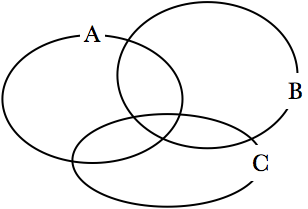
\includegraphics[scale=0.35]{FiguresMaths/3sets}
    \caption{Three sets, $A$, $B$ and $C$, in ``general" position, i.e., with all possible overlaps.}
        \label{fig:unionSetsInit}
\end{center}
\end{figure}
\begin{figure}[htb]
\begin{center}
        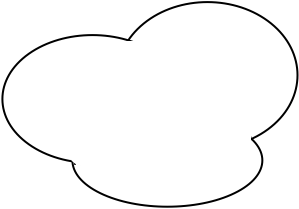
\includegraphics[scale=0.35]{FiguresMaths/RuleAdditive}
        \hspace{1cm}
        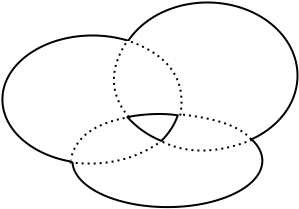
\includegraphics[scale=0.35]{FiguresMaths/RuleAdditive2}
        \caption{The union of sets $A$, $B$, and $C$ (left), and their intersections (right).}
        \label{fig:unionSets}
\end{center}
\end{figure}
In order to draw explicit expressions that express the content of  Fig.~\ref{fig:unionSets}, one must apply the law of {\em inclusion and exclusion} in multiple ways, as we compensate for the 
pairwise and triple intersections among  sets $A$, $B$, and $C$.  A careful reckoning using the figure indicates that
\[ |A \cup B \cup C| \ \ = \ \ 
\big(|A| + |B| + |C| \big) - \big( |A \cap B| + |A \cap C| + |B \cap C| \big) + |A \cap B \cap C|. \]
In particular, we begin by {\em including} the union; then we {\em exclude} the pairwise intersections, which were double-counted; and we finally {\em include} the triple intersection, which was first counted three times and then excluded three times while
removing the pairwise intersections.

\medskip\item
{\em The multiplication rule} \index{The multiplication rule for counting elements of sets}

\smallskip

This rule tells us how to count the cardinalities of Cartesian products of sets, as illustrated in Fig.~\ref{fig:cartesianproduct}.
\[ |A \times B| \ \ = \ \ |A| \cdot |B| \]
The multiplication rule extends immediately to multiplicities of sets; e.g., for three sets:
\[  |A \times B \times C| \ \ = \ \ |A| \cdot |B| \cdot |C| \]

\smallskip

As an important special case, we note that
\[ |A \times A \times \cdots  \times A| \ \mbox{ ($p$ occurrences of $A$)}  \ \ = \ \ |A|^p \]
The exciting feature in this last equality is that the set
 \[ A \times A \times \cdots  \times A  ~~\mbox{($p$ occurrences of $A$)} \]
is a (nonstandard) way of representing the set of length-$p$ strings of elements of $A$.  Thereby, the multiplication rule gives us an alternative way to  view---and to prove---Proposition~\ref{thm:b-ary strings}.
\end{itemize}

\bigskip

As we move forward, we shall encounter many other ways of counting the elements of sets,
most importantly by using operations involving {\it selection} and {\it rearrangement}.  As we
proceed with this new material, we will encounter old friends, often wearing new clothing.  We
will renew our acquaintance with the factorial operation and with binomial coefficients; we will
have cause to recall the pigeonhole principle in new settings.  And, we will discover new domains of application, as we move beyond ``pure" mathematics to the applications of mathematical laws in domains related to probability and statistics.

\smallskip

Let us begin our journey.

\subsection{Counting Based on Set Arrangement and Selection}
\label{sec:set-arrangement}

This section introduces the primary operations that are used for arranging finite sets as we
establish a base for studying combinatorial probability.  The importance of set-arrangement
in this context results from the common practice of defining discrete probability/likelihood as a counting problem---most specifically, of defining the ratio
\begin{equation}
\label{eq:prob-def-ratio}
\frac{\mbox{number of ways of achieving a targeted event $E$}}{\mbox{number of possible events}}
\end{equation}
as the {\it probability of event} $E$.

\index{probability of event $E$}

\medskip

We focus on three notions of arranging, and selecting from, a set of $n$ objects:
\[ \{ x_1, x_2, \ldots , x_n\} \]
When useful for explaining some idea, we sometimes identify the $x_i$ as some specific type
of objects, such as numbers, but generally we do not exploit any specific characteristics of the $x_i$.

\medskip

\index{permutation}

\noindent {\it Permutations}.
A permutation of an $n$-element set $A$ is a {\em fixed ordering} of the elements of $A$: each element of $A$ appears precisely once in the ordering.  We denote a permutation of an $n$-element set via the notation
\[ (x_1, x_2, \ldots , x_n) \]
where each $x_i$ appears precisely once.  Note that we use parentheses for grouping, as in ``$(3,2,1,4)$", instead of braces, as in ``$\{3,2,1,4\}$", to emphasize the ordering.  In particular,
\[ \{3,2,1,4\} \ = \ \{1,2,3, 4\} \ \ \ \ \mbox{ but } \ \ \ \ (3,2,1,4) \ \neq \ (1, 2, 3,4) \]

\medskip

\index{selection problems}

In terms of problems relating to {\em selecting} $m$ elements from a set of $n \geq m$ elements, permutations give rise to the most demanding genre of selection: {\em They demand accounting for both the {\em identities} of the selected elements and the {\em orders} in which the elements were selected.}

\medskip

It is a straightforward exercise to count the number of permutations of $n$ items.

\begin{prop}
\label{thm:no-permutation}
The number of permutations, $P(n)$, of a $n$-element set equals $n!$
\end{prop}

\begin{proof}
Just for the practice, we describe two inductive proofs of this simple result, based on two quite-distinct ways of constructing permutations.  We merely sketch the inductions underlying the proofs, leaving details for the reader.

\medskip

\noindent {\bf 1.}
To construct a permutation of the $n$-element set $\{ x_1, x_2, \ldots , x_n\}$:
\begin{itemize}
\item
We can select the first element of the permutation in $n$ ways: any $x_i$ will work.
\medskip\item
Having selected the first item, we are left with the $(n-1)$-element version of the problem.
\end{itemize}
We thereby find that $P(n)$ is specified recursively as follows.
\[
P(n) \ = \ \left\{
\begin{array}{cl}
1 & \mbox{ if } \ n=1 \\
n \times P(n-1) & \mbox{ if } \ n>1
\end{array}
\right.
\]
By elementary reasoning, we find that $P(n) \ = \ n!$

\bigskip

\noindent {\bf 2.}
To construct a permutation of the $n$-element set $A = \{ x_1, x_2, \ldots , x_n\}$:
\begin{itemize}
\item
Assume, inductively, that you are given a fixed  permutation $(x_1, \ldots , x_{n-1})$ of an $(n-1)$-element subset $A'  \subset A$, chosen somehow from among the $(n-1)!$ possible orderings of set $A'$.  (Note the thinly veiled use of induction.)
\medskip\item
Take element $x_n$, which does not belong to $A'$, and place it into the ordering of $A'$ that you are given.  You can place $x_n$ in any of $n$ positions in the new permutation:
  \begin{itemize}
  \item
before (i.e., to the left of) all of the already placed elements of $A'$;
  \medskip\item
after (i.e., to the right of) all of the already placed elements of $A'$;
  \medskip\item
in between any adjacent already placed elements of $A'$.
  \end{itemize}
Each of the preceding $n$ choices creates a unique permutation of the $n$-element set $A$.
\end{itemize}
Using arithmetic virtually identical to case {\bf 1}, we verify that $P(n) \ = \ n!$.

\medskip

\noindent
Other variants on the preceding proof themes will undoubtedly occur to you.   \qed
\end{proof}

%%%%%%%%%%%%%%%%%%%%%%%

\medskip

\noindent {\it Combinations}.\index{combination}
Within the context of selection problems, combinations are the ``next step down" in strictness from permutations.  When one selects $m$ items from a set of $n \geq m$ items, combinations are concerned with the {\em identities} of the elements selected, but not with the order in which their elements are chosen.

\smallskip

\noindent (This willingness to ignore order gives a big hint about how to count the number of
combinations of $m$ items chosen from $n$.  Can you figure out how to use the hint before
we get to Proposition~\ref{thm:no-combination}?)

\medskip

Factorials play as essential a role in combinational selection as in permutational selection, but
now it plays a {\em dual} role: choosing the identities of the selected elements {\em and} factoring out the order in which the elements were selected.  The binomial coefficients that we introduced in Section~\ref{sec:binomial-coeff} and that have arisen several times since then
throughout our journey are (literally!) tailor made for this genre of selection problem.  Recall that
\[ {n \choose m} \ = \ \frac{n \times (n-1) \times \cdots \times (n-m)}{m!} \ = \  \frac{n!}{m!(n-m)!} 
\]

\begin{prop}
\label{thm:no-combination}
The number of ways of selecting $m$ elements from a set of $n \geq m$ elements, while ignoring the order in which the $m$ elements were selected is $\displaystyle {n \choose m}$.
\end{prop}

\begin{proof}
The number of {\em ordered} ways of selecting $m$ elements from a set of $n \geq m$ elements is 
\begin{equation}
\label{eq:combination}
n \times (n-1) \times \cdots \times (n-m+1) \ = \ \frac{n!}{(n-m)!}
\end{equation}
To wit: One can select the first element in any of $n$ ways.  Having selected this element, there are: $n-1$ ways to choose the second element; $n-2$ ways to choose the third element; $n-3$ ways to choose the fourth element; and so on.

\smallskip

There is a bit of complexity here, so let us say the same thing in a few ways:

\noindent
This method of numeration accounts for both the identities of the $m$ elements and the order in which they are selected.  For each position $i$, the method accounts for both the identity of the $i$th chosen element {\em and} the fact that it was the $i$th element chosen.  In more detail, if element $x_1$ is the first element chosen, and element $x_2$ is the second one chosen, then the two orders of selection
\[ x_1, \ x_2, \ \mbox{(some fixed order for the remaining $m-2$ selections)} \]
and 
\[ x_2, \ x_1, \ \mbox{(some fixed order for the remaining $m-2$ selections)} \]
are counted as separate events.  Easily, this overcounting uniformly
expands each of the events that we {\em do} want to account for by the
factor $m!$, for this is the number of orders in which we could have selected the finally chosen $m$ elements.

\smallskip

This reasoning indicates that we can compensate for our overcounting by dividing the {\em ordered} tally (\ref{eq:combination}) by $m!$.  This compensation replaces tally (\ref{eq:combination}) by the binomial coefficient $\displaystyle {n \choose m}$, whence the result.  \qed
\end{proof}

\bigskip

\noindent \fbox{
\begin{minipage}{0.96\textwidth}
{\bf Explanatory note}.

\smallskip

Binomial coefficients have thus made yet another appearance in our journey!  The many situations that are counted by this construct are only suggested by their occurrence here, in respect to probabilities, as well as in Chapter~\ref{ch:Summation} within the context of evaluating summations and in Chapter~\ref{ch:Recurrences} within the context of solving recurrences.  The multiple occurrences of binomial coefficients within these apparently unrelated contexts provide a powerful argument for the value of abstracting beyond the superficial details of phenomena in the direction of their deep essentials.  This insight will only be reinforced as we proceed with our study of combinatorial probabilities.
\end{minipage}
}

\bigskip

\index{derangement} \index{avoidance problems}

\noindent {\it Derangements}.
Derangements represent one of the simplest forms of {\em avoidance problems}.  Here is a
well-known version of such a problem, in preparation for the general definition.

\smallskip

Professor $X$ views it as a win-win strategy for the students in her class to grade each others' essays on {\it The Essential Truth in the Universe}.  The essays thereby get graded faster, because the grading process becomes a parallel rather than sequential process.  Moreover, each student gets a chance to see how another student has interpreted some basic component of the human experience.  The only complication is: How should Professor $X$  allocate essays among the students.  {\em The process must ensure that no student is assigned her own essay to critique.}

\smallskip

The challenge that Professor $X$ is facing is known as a {\em derangement problem}.

\bigskip

\noindent 
A {\em derangement} of a (finite) set $A$ is a {\em bijection} $f: A \leftrightarrow A$ that has no 
{\em fixed point}.  In other words, for every $a \in A$, we must have $f(a) \neq a$.

\medskip

Clearly, derangements always exist (for $n>1$).  One can just label the elements of set $A$ by the numbers $0, 1, \ldots, |A|-1$ and specify $f(a) = a+1 \bmod |A|$.

\medskip

But, playing around with some sets should convince you that derangements are not so common!
In fact, the set  $A = \{0, 1,2 \}$ admits $6$ self-bijections, but only two are derangements, namely:
\[
\begin{array}{lll}
f(a) = a+1 \bmod 3 &: \mbox{which maps} &(0 \rightarrow 1),  (1 \rightarrow 2), (2 \rightarrow 0) \\
\mbox{and} &  & \\
g(a) = a-1 \bmod 3 &: \mbox{which maps} & (0 \rightarrow 2),  (1 \rightarrow 0), (2 \rightarrow 1)
\end{array}
\]

\medskip

How many derangements does an arbitrary $n$-element set $A$ have?   We denote this quantity by $d(n)$.

\smallskip

While the general problem of counting derangements is beyond the scope of an introductory text, the reader will benefit from observing the process of deriving a recurrence for $d(n)$.  

\medskip

We compute $d(n)$ for arbitrary $n \in \N^+$ via the following recursion:
\begin{itemize}
\item
For $n=1$:  \ $d(1) = 0$.

\smallskip

To wit, the unique bijection in this case consists only of a fixed point. 

\medskip\item
For $n=2$:  \ $d(2) = 1$.

\smallskip

There are two bijections in this case, the identity, which has two fixed points, and the swap,
which is a derangement.

\medskip\item
For $n > 2$: \ $d(n) = (n-1) (d(n-1) + d(n-2))$:

\smallskip

To see this, note first that in any derangement, the first element of $A$, call it $a$, must map to some $b \neq a$.

\smallskip

Note next that there are $n-1$ ways to choose $b$.
  \begin{itemize}
  \item
There are $d(n-2)$ derangements under which $b$ maps to $a$.  In those cases, we know everything about $a$ and $b$, so we need worry only about the remaining elements of $A$.  These $n-2$ elements can ``derange" in all possible ways.

  \medskip\item
There are $d(n-1)$ derangements under which element $b$ does not map to $a$.  In detail,
as the process of ``choosing an image" passes through $A$, every element has two forbidden
choices: it cannot choose itself (for that would be a fixed point) and it cannot choose one other
element (for element $b$, this is element $a$).  In some sense, the notion of a forbidden element gets passed around, changing its identity at every step.
  \end{itemize}
%$d(n) = (-1)^n + n d(n-1)$
\end{itemize}
The preceding reasoning verifies the following recurrence
\[
d(n) \ = \ \left\{
\begin{array}{ccl}
0 &  & \mbox{ if } n=1 \\
1 &  & \mbox{ if } n= 2 \\
(n-1) (d(n-1) + d(n-2)) &  & \mbox{ if } n> 2
\end{array}
\right. 
\]

\medskip

Interestingly, as the number of objects in the set to be deranged grows without bound, the
proportion of bijections that are derangements tends to the limit $1/e$, where $e$ is Euler's
constant (the base of natural logarithms).

\section{Introducing Combinatorial Probability via Examples}
\label{sec:combinatorial-prob}

\index{probability via counting} \index{game of poker}

Perhaps the easiest and most engaging way to introduce ``combinatorial probability''---i.e., probability via counting"---is by calculating game-related likelihoods---deals of cards, rolls of dice, and guessing games of various sorts.  Why is one specific genre of deal in the game of poker (say, a ``straight") worth more than another (say, ``three of a kind")?  The arithmetic required for such a discussion is elementary, and the references to {\it gedanken gambling} (gambling via thought experiment) are easily understood---and, they are usually of some interest even to non-gamblers.  One can also introduce in such a setting concepts such as randomness and bias, which are so important in the design of experiments and the analysis of their outcomes.

\smallskip

This, then, will be our approach to the subject of combinatorial probability.  The reader has already seen more than enough ``dry" facts about sets and how to count their elements.  It is time to reap some rewards from the work of acquiring that knowledge. 

\ignore{***************
\subsection{A Practical Introduction to Probability}
\label{sec:prob-stat}

Elements of probability theory and statistics infuse every area of
computing.  The practicality of many algorithms that are
experientially the most efficient for their target tasks depend on the
{\em distribution} of inputs in ``real" situations.  Design
methodologies for crucial complex circuits must acknowledge the {\em
  mean times to failure} of the critical components of the circuits.
Sophisticated searching algorithms must take into account the relative
{\em likelihoods} of finding one's goal in the various optional search
directions.  Analyzing and understanding large corpora of data
requires a variety of methodologies that build on the concepts of {\em
  clustering} and/or {\em decomposition}.

A student needs at least an introduction to the foundations of
probability and statistics to even understand, all the more so to
master, the terms highlighted in the preceding paragraph.  We outline
many of the key concepts that a student must be exposed to in the
following subsections.

{\Denis Here we may be more precise about the content: the probabilities are built upon combinatoric rules, another interesting point is to distinguish between probability and statistics...}
*****************}

\bigskip

Before we begin to play, though, we need some groundwork, beginning with the combinatorics-based definition of ``probability'' that sets the tone for this section.

\medskip

\noindent
As noted earlier, the {\em (discrete) probability}, or, {\em likelihood}, of an event is given by the ratio (\ref{eq:prob-def-ratio}), which measures the number of targeted events as a fraction of the number of possible events.

\smallskip

\noindent
This approach to ({\em discrete}) probabilities has important technical consequences.\footnote{We emphasize the word ``discrete" because the asserted dichotomy does not generally hold in the world of events that assume continuous values.}
  \begin{itemize}
  \item
The probability of any targeted event $E$ is $\leq 1$.  This means:
    \begin{itemize}
    \item
If the probability of $E$ is $1$, then event $E$ is a {\em certainty}.
    \medskip\item
If the probability of $E$ is $< 1$, then event $E$ is possible but not certain.
   \end{itemize}

 \medskip\item
The probability of any targeted event is $\geq 0$.   This means:
    \begin{itemize}
    \item
If the probability of $E$ is $0$, then event $E$ is an {\em impossibility}.
    \medskip\item
If the probability of $E$ is $> 0$, then event $E$ is a possibility.
   \end{itemize}

  \medskip\item
The more likely event $E$ is, the closer its probability is to $1$.
  \medskip\item
By the addition rule for counting sets, the joint probability of two {\em disjoint} events equals the sum of the events' probabilities.
  \medskip\item
As a special case of the preceding rule: the joint probability of two {\em complementary} events
equals $1$.  This is because the complement of an event whose probability is $p$ has
probability  $(1-p)$.
  \end{itemize}

\bigskip

\noindent \fbox{
\begin{minipage}{0.96\textwidth}
{\bf Explanatory note}.

\smallskip

In our formulation, a probability as a number $p$ in the range $0 \leq p \leq 1$.  

\smallskip

It is also very common, though, to view a probability as a {\em percent}, as in

\smallskip

\hspace*{.2in}``The likelihood of rain this morning is $50$\%."

\medskip

In order to understand these alternative locutions, the reader should recall that the word ``percent" derives from the Latin ``{\it per centum}", which means ``per hundred".  Therefore, one can always interchange the following  locutions

\smallskip

\hspace*{.2in}``Event $E$ occurs with probability $p$."

\hspace*{.2in}``Event $E$ occurs with probability $(100 p)$\%."
\end{minipage}
}

\bigskip

\noindent
We are going to focus on {\em games of pure chance}---with no complicating notion of strategy---because our underlying interest is in probability, not game theory.

\bigskip

\noindent \fbox{
\begin{minipage}{0.96\textwidth}
{\bf Enrichment note}.

\smallskip

There exists an exciting mathematical field of study that is dedicated to all games: games of pure chance (which is our focus), games that combine skill and chance (e.g., {\it backgammon} or {\it bridge} or {\it poker}), and games of pure skill (e.g., {\it chess} or {\it GO}).   But, alas, the issues that one must deal with when studying the broad spectrum of games go beyond the  scope of our introductory text.

\medskip

\index{von Neumann, John} \index{Morgenstern, Oskar} \index{Nash, John}

We recommend to the reader just two classical works that may be of interest for historical and cultural reasons, as well to supply a foundation for further study.  The first reference is to the
classic \cite{vonNeumann-Morg} by American polymath John von Neumann  and German economist Oskar Morgenstern, which established the connection between the mathematical subject of game theory and the field of economics.  (Now-familiar concepts such as ``rational game" and ``zero-sum game" originated in \cite{vonNeumann-Morg}.)  The second classic is \cite{Nash50}, by the American mathematician John Nash, which introduced the now-familiar notion of ``Nash equilibrium." (The story behind \cite{Nash50} is movingly related in the movie ``{\it A Beautiful Mind}".)
\end{minipage}
}


\subsection{The Game of Poker: Counting Joint Events}

We focus on a typical deck of 52 playing cards: The cards are partitioned into

\medskip

\noindent
\begin{tabular}{cll}
$*$ &
four {\em suits}:  & {\sc clubs}, {\sc diamonds}, {\sc hearts}, {\sc spades} \ (in increasing value) \\
  \\
$*$ &
$13$ {\em face values}: &
$\displaystyle \left\{
\begin{array}{l}
\mbox{number cards}: 
2, 3, 4, 5, 6, 7, 8, 9, 10 \\
\mbox{picture cards}: 
\mbox{{\sc Jack, Queen, King, Ace}  (in increasing value)}
\end{array}
\right.$ 
\end{tabular} 

\medskip

\index{the number of random $5$-card deals in poker} 

\noindent
In a popular version of the game of poker, each player is dealt a {\it hand} consisting of five cards.  The total number of possible $5$-card hands, i.e., of (unordered sets) of $5$ cards, is just the number of ways of choosing a $5$-element set from a $52$-element set.  Invoking the counting techniques from Section~\ref{sec:set-arrangement}, we note that this ``astronomical" number is
\[
{32 \choose 5} \ \ = \ \ \frac{52!}{5! 47!} \ \ = \ \ 2,598,960 
\]
The size of this number explains much of what of makes the game of poker so interesting.

\medskip

Of course, it is the {\em patterns} of the cards in various hands that determines which hands beat other ones in the competition that is at the heart of poker.  It is a reasonable conjecture that

\smallskip

{\em
\begin{tabular}{l}
{\bf Conjecture}.
The value of a pattern in poker accurately tracks the likelihood \\
of a player's receiving the pattern in a random deal.
\end{tabular}
}

\smallskip

\noindent
(Of course, {\em random} deals are the embodiment of a {\em fair} game.)

\bigskip

We now calculate the likelihoods of a variety of patterns' arising in a fair game of poker, in order to study the validity of the preceding conjecture.  As we derive the likelihoods of the various patterns, observe the many invocations of the multiplication rule for the probabilities of independent events.

\medskip

\index{royal flush (in poker)} \index{straight flush (in poker)}
\begin{itemize}
\item
A {\it royal flush} is a poker hand of the form

\smallskip

\hspace*{.25in}$10$, \ {\sc Jack}, \ {\sc Queen}, \ {\sc King}, \ {\sc Ace} \ \ of the same suit

\smallskip

\noindent
There are only four ways to form a royal flush---one for each suit.  Therefore, the probability that
a fair deal will produce such a hand is
\[ 
Pr(\mbox{royal flush}) \ \ = \ \
\frac{4}{2,598,960} \ \ = \ \ {1 \over {649,740}} \ \ \approx \ \ 0.00000154 \ \ = \ \ 1.54 \times 10^{-6} \]

\medskip\item
A {\it straight flush} is a poker hand in which the cards share the same suit and follow one 
another in value.  Thus, a royal flush is a straight flush whose highest-rank card is an {\sc Ace}.

\medskip

Let us calculate the number of straight flushes.

\smallskip

The counting is similar to that for a royal flush:  For each suit, there are nine sequences of $5$ cards that are consecutive in rank.  From lowest rank to highest:
\[ \begin{array}{llccccc}
\mbox{Hand \#1}: & &
2 & 3 & 4 & 5 & 6 \\
\mbox{Hand \#2}: & &
3 & 4 & 5 & 6 & 7 \\
\mbox{Hand \#3}: & &
4 & 5 & 6 & 7 & 8 \\
\mbox{Hand \#4}: & &
5 & 6 & 7 & 8 & 9 \\
\mbox{Hand \#5}: & &
6 & 7 & 8 & 9 & 10 \\
\mbox{Hand \#6}: & &
7 & 8 & 9 & 10 &  \mbox{J} \\
\mbox{Hand \#7}: & &
8 & 9 & 10 &  \mbox{J} &   \mbox{Q} \\
\mbox{Hand \#8}: & &
9 & 10 &  \mbox{J} & \mbox{Q} &  \mbox{K}  \\
\mbox{Hand \#9}: & &
10 &  \mbox{J}
     & \mbox{Q}
     & \mbox{K}
     & \mbox{A}
\end{array} \]
The probability of being dealt a royal flush is, thus, precisely $1/9$ the probability of being dealt a straight flush.  The probability of getting a straight flush is, therefore,
\[  Pr(\mbox{straight flush}) \ \ = \ \
{9 \over {649,740}} \ \ \approx \ \ 0.0000139  \ \ = \ \ 1.39 \times 10^{-5} \]

\medskip\item
{\it Four-of-a-kind} is a poker hand of the form

\smallskip

\hspace*{.25in}$X, \ X, \ X, \ X, \ Y$

\smallskip

where $X, Y \in \{2, \ 3, \ 4, \ 5, \ 6, \ 7, \ 8, \ 9, \ 10, \ \mbox{J}, \ \mbox{Q}, \ \mbox{K}, \ \mbox{A}\}$, 
and $X \neq Y$.
\index{four of a kind (in poker)}

\medskip

There are $13$ possible face values; each is a candidate for being card $X$.  Having chosen card $X$, there are $48$ possible choices for card $Y$.  Each selection  of cards $X$ and $Y$ specifies a unique {\it four-of-a-kind} poker hand.  The multiplication principle thus tells us that there are precisely $13 \times 48 = 624$ {\it four-of-a-kind} poker hands, so the probability of being dealt such a hand is
\[ 
Pr(\mbox{four of a kind}) \ \ = \ \
\frac{624}{2,598,960 }  \ \ \approx \ \ 2.4 \times 10^{-4} . \]

\ignore{***********
is a remaining card left that is any one among the 48 remaining ones.
Indeed, according to the multiplicative principle, it remains ${12 \choose 1}$ in each of the $4$ colors. 
Thus, $13 \times 48 = 624$, which corresponds to the probability $0.00256$.
*************}

\medskip\item
We look at the next two poker hands together because the analyses of their respective patterns are so similar.
\begin{itemize}
\item
A {\it Full house} is a poker hand of the form

\smallskip

\hspace*{.25in}$X, \ X, \ X, \ Y ,\ Y$

\smallskip

where $X, Y \in \{2, \ 3, \ 4, \ 5, \ 6, \ 7, \ 8, \ 9, \ 10, \ \mbox{J}, \ \mbox{Q}, \ \mbox{K}, \ \mbox{A}\}$,  and $X \neq Y$.
 \index{full house (in poker)} 

\medskip\item
{\it Three of a kind} is a poker hand of the form
\index{three of a kind (in poker)}

\smallskip

\hspace*{.25in}$X, \ X, \ X, \ Y, \ Z$

\smallskip

where $X, Y,  Z \in \{2, \ 3, \ 4, \ 5, \ 6, \ 7, \ 8, \ 9, \ 10, \ \mbox{J}, \ \mbox{Q}, \ \mbox{K}, \ \mbox{A}\}$,  and $|\{X, Y, Z\}| =3$.  The final equation, about set-cardinality, is a ``cute", succinct, way of saying that $Y$ and $Z$ differ both from $X$ and from each other.
\end{itemize}
For both of these patterns, the analysis begins by noting that the face-value $X$ can be chosen
in $13$ ways.  Having chosen face-value $X$, we select three of the four cards with that face-value: this choice can be made in $\displaystyle {4 \choose 3} = 4$ ways.  The $X$ component of the hand has now been selected.

\smallskip

With the {\it full-house} pattern, we must now choose the face-value $Y$.  This can be done in $12$ ways.  The selection of the hand is completed once we select the $\displaystyle {4 \choose 2} = 6$ needed cards that have face-value $Y$.

\smallskip

Summing up, the {\it full-house} pattern can be assembled in
\[ 13 \cdot {4 \choose 3} \cdot 12 \cdot {4 \choose 2} \ \ = \ \  3,744 \]
ways, so the probability of being dealt such a hand is
\[ 
Pr(\mbox{full house}) \ \ = \ \
\frac{3744}{2,598960}  \ \ \approx \ \ 1.44 \times 10^{-3}
\]

\medskip

To finish up the {\it three-of-a-kind} poker hand, we remark that once we have selected the $X$
component of the hand, we must select the remaining cards by choosing the (distinct) face-values of $Y$ and $Z$; this can be done in $\displaystyle {12 \choose 2} = 66$ ways.  Then, for each of these choices we must select a specific card, which can be done in $4$ ways.  We thereby find that the {\it three-of-a-kind} pattern can be assembled in
\[ 13 \cdot {4 \choose 3} \cdot {12 \choose 2} \cdot 4^2 \ \ = \ \  54,912 \]
ways, so the probability of being dealt such a hand is
\[ Pr(\mbox{three of a kind}) \ \ = \ \
 \frac{54,912}{2,598,960}  \ \ \approx \ \ 2.11 \times 10^{-2}  \]

\medskip\item
The final poker hand that we consider is {\it two-pair}.  We remarked earlier in this section that three-of-a-kind beats two-pair.  Comparing the likelihood of two-pair versus the just-computed likelihood of three-of-a-kind will be a good test of our poker-valuation conjecture.
\index{two-pair (in poker)}

\smallskip

The {\it two-pair} hand in poker is a deal that is {\em a permutation of} the hand
\[ X, \ X, \ Y, \ Y, \ Z \]
where $X$, $Y$, $Z$, are distinct face values.

\smallskip

You can show ({\em in a exercise}) that the probability of receiving a two-pair hand in a fair poker deal is
\[ Pr(\mbox{two-pair}) \ = \ \frac{123,552}{2, 598, 960} \ \approx \ 4.75  \times 10^{-2} \]
This is a bit more than twice the probability of receiving a three-of-a-kind---which explains why the latter hands beats the current one in a poker game.
\end{itemize}

\medskip

One can find in many sources (including the Internet) tables that: enumerate all possible poker hands; describe all ways of assembling each hand; compute the probabilities of being dealt each hand.

\smallskip

Of course, our interest has been in exposing how to perform these calculations, not with their
results---but it s fun to see why the various poker hands have their relative values in the game.


\subsection{The Monty Hall Puzzle: {\em Conditional} Probabilities}
\label{sec:monty-hall}

The following real-life situation illustrates that reasoning probabilistically is not easy and that it can be quite unintuitive.

\bigskip

\index{Let's Make a Deal}

We recall a popular TV show from the 1970s and 1980s, \textit{Let's Make a Deal}.  In one segment of each episode of the show, a contestant was confronted by three doors: door (1), door (2), and door (3) in Fig.~\ref{fig:MonthyHal-1}.
\begin{figure}[htb]
\begin{center}
        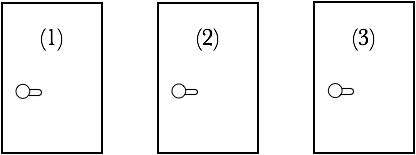
\includegraphics[scale=0.4]{FiguresMaths/MonthyHallInitial}
        \caption{The three doors of \textit{Let's Make a Deal}.}
        \label{fig:MonthyHal-1}
\end{center}
\end{figure}
The contestant was told that a jackpot was hidden behind one of the doors and that the other two doors hid less-desirable outcomes.  The show's host, Monty Hall, invited the contestant to choose one of the doors: the contestant would receive whatever prize was behind the selected door.
\index{Hall, Monty} 

\smallskip

Since the doors' names are irrelevant to the story, let us assume that the contestant chose door (3).  Before that selection was considered final, Monty Hall would open {\em one of} doors (1) or (2), i.e., one of the two {\em unchosen} doors.  Monty made sure---unbeknownst to the contestant---to choose a door that did {\em not} hide the jackpot.  Again for illustration, let us assume that Monty opened door (1).  When the jackpot did not appear  behind door (1), Monty now gave the contestant the option of changing her initial choice, from door (3) to door (2).

\medskip

What should the contestant do?  

\medskip

Let us begin with intuition.  As the story began, the contestant had a one-in-three chance of choosing the door that hid the jackpot.  As the story progresses, is it conceivable that these odds could have changed after door (1) is shown {\em not} to hide the jackpot?  How could this be?

\smallskip

\index{vos Savant, Marilyn}
Well, the popular (well-named) newspaper columnist Marilyn vos Savant published an analysis that shows that {\em it is better to change one's choice!}  Here is her reasoning, enhanced by the illustration in Fig.~\ref{fig:MonthyHall-2}.
\begin{figure}[htb]
\begin{center}
        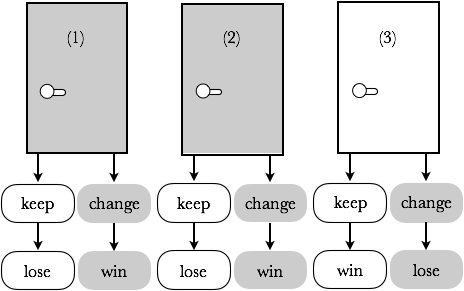
\includegraphics[scale=0.4]{FiguresMaths/MonthyHall}
        \caption{Suppose the jackpot is behind door (3).  If the contestant selected door (3) initially, then {\em not switching is a win}, while {\em switching is a loss}.  If the contestant selected either door (1) or door (2) initially, then {\em switching is a win}, while {\em not switching is a loss}.}
        \label{fig:MonthyHall-2}
\end{center}
\end{figure}
There are two possible cases.
\begin{itemize}
\item
If the contestant had selected the jackpot-door initially, then holding on to this choice leads to the same probability of success as she had from the beginning, namely, $1/3$.
\medskip\item
If the contestant had selected a wrong door initially---which occurs with probability $2/3$---then she will win the jackpot if she now changes her initial (erroneous) choice.
\end{itemize}
Thus, quite unintuitively, the probabilities {\em have changed}, and the contestant should change her original choice based on the information she has now.

\smallskip

You can have fun by confronting your friends with this unintuitive analysis.

\medskip

\index{conditional probability} \index{Bayes's Theorem}

Of course, the Monty Hall game and its analysis are not just a trick!  Our story is a demonstration that you can improve your chances of winning by taking advantage of all available information!  The ``science'' behind this analysis builds upon the topic of {\em conditional probability}.  Rather than looking only at the probability of an event $E$ in isolation, one focuses on the probability of event $E$, {\em given that some event $F$ has occurred}.  The {\em notation} that traditionally indicates this shift in focus is the following: If one uses the notation $Pr[E]$ to denote the probability of event $E$ in isolation, then one uses the embellishment $Pr[E \ | \ F]$ to denote, the probability of the compound event: ``$E$, given $F$''.

\medskip

In order to supply a complete development of the theory that explains the Monty Hall puzzle, we would have to employ conditional probabilities, which would require invoking Bayes's Theorem, a seminal result within the theory of conditional probabilities---which would take us beyond the limits of an introductory text.

\smallskip

We refer the interested reader to \cite{Lee12} for a general presentation of this area, and to \cite{Bayes} for the original work on the Theorem.

\smallskip

And---see the interactive sites on the Internet that interactively perform the computation of (conditional) likelihoods!


\subsection{The Birthday Puzzle: {\em Complementary} Counting}
\label{sec:birthday-puzzle}
\index{birthday puzzle}

This section presents another application of the rules of enumeration to the calculation of probabilities.  The main lesson associated with this application is the following.

\smallskip

\noindent
{\em it is sometimes easier to calculate the probability that event $E$ {\em does not} occur than the probability that it {\em does} occur.}  

\smallskip

\noindent
(Of course, this is not a formal  proposition. But, we do invite you to replicate the conclusions of this section via a direct argument.)

\bigskip

A common technique that teachers employ to establish rapport with a new class is to determine whether any students in the class share a birthday.  We now demonstrate that when the class has (at least) around 30 students, the answer is usually \textit{yes}.  The fact that we can make such a specific claim suggests that the presence of birthday-sharers is not a mere accident---there are probabilities at work here!

\medskip

\noindent
We study the following question.

\smallskip

{\it How many people must gather before the probability that some two share}

{\it a birthday reaches 50\%?}

\medskip

\noindent
We develop an answer to this question, based on the assumption that all dates are equally probable potential birthdays.

\bigskip

Let us focus on a common year, with 365 days; a simple modification of the coming calculation 
accommodates leap years.  A first, obvious, remark is that when there are 366 people in the 
class---and only then---the pigeonhole principle {\em guarantees} (with probability 100\%)  that some two people share a birthday.  When we lower our birthday-sharing target to a  {\em 50\% probability} of a shared birthday, how much does this lower the required population  of 366?  Somewhat unintuitively, the required number is lowered dramatically!

\bigskip

\index{dual problem} 
We simplify the calculational component of our solution considerably by focusing on the  {\em dual} form of our problem.  That is:

\begin{description}
\item[]
{\em Instead of} determining a {\em lower bound} on the population that would guarantee a 50\% probability of a shared birthday,

\medskip\item[]
{\em we determine} an {\em upper bound} on the population that would guarantee a 50\% probability of {\em no} shared birthday.
\end{description}

\smallskip

Since we assume that all birthdays are equally likely, the probability that any particular person has any particular birthday is $1/365$.  In other words, the space of all possible assignments of birthdays to all $n$ people has $365^n$ assignments---all of which are equally likely.

\bigskip

Let us perform the following {\em gedanken} assignment of birthdays.

\smallskip

Say that we have an assemblage of $n$ ``proto-people"---i.e., people who do not yet have  birthdays.  Our task is to assign birthdays to these folks in such a way that no two of them share a birthday.
\begin{itemize}
\item
We can select a birthday for person \#1 from any of the $365$ (indistinguishable) days of the year.
\medskip\item
We can select a birthday for person \#2 only from the $364$ (indistinguishable) days of the year that person \#1 has not ``occupied''.

\smallskip

Otherwise persons \#1 and \#2 would share a birthday!
\medskip\item
Proceeding by similar reasoning:  We can select person \#3's birthday from only the $363$ days that the first two people have not ``occupied"; we have $362$ days available for person \#4, and so on, until person \#$n$'s birthday must be selected from among $365-(n-1)$ days.
\end{itemize}
Our procedure indicates that among the $365^n$ possible assignments of birthdays to $n$ people, only
\[ 365 \times 364 \times 363 \times \cdots \times (366-n+1) \ = \ \frac{365!}{(365-n)!}  \]
assignments have no two people sharing a birthday.

\smallskip

Worded as a probability: Letting $Pr(n)$ denote the probability that there are no shared birthdays in a population of $n$ people:
\begin{eqnarray*}
Pr(n) & = &
\frac{\mbox{number of birthday assignments with no shared birthday}}
{\mbox{total number of birthday assignments}} \\
 &  = & \frac{365!}{ (365-n)!  \times 365^n} \\
 & = & \frac{n!}{365^n} {365 \choose n}
\end{eqnarray*}

\medskip

Let us return to our original problem, which focuses on assignments in which there exists at least one shared birthday.  Since the event

\smallskip

\hspace*{.25in}some two people share a birthday

\smallskip

\noindent
is the complement of the event

\smallskip

\hspace*{.25in}no two people share a birthday

\smallskip

\noindent
the probability of a shared birthday is precisely $1-Pr(n)$.  For $n=23$, the desired probability is $0.5073$:  In other words,

\begin{prop}
In any group of $23$ people, the likelihood that two people share the same birthday is slightly greater than $50\%$, assuming a year with $365$ equally likely days.
\end{prop}

When our teacher's class grows to 30 students, the probability of a shared birthday grows to $70.632\%$.


\subsection{Sum-of-Spots Dice Games: Counting with Complex Events}
\label{sec:three-dice}
\index{Dice games}

Archaeology suggests that games have fascinated our species since our origins.  The 
games that have endured span a spectrum from those that depend almost entirely on thinking and strategy to those that depend on pure chance.  A number of games that have endured involve the rolling of 6-sided dice, each die\footnote{The word ``dice'' is plural; the singular form is ``die''.}~having distinct numbers (usually denoted by {\it spots}) on its six faces.  For convenience, we refer to each die's face-numbers via the numerals $1, 2, 3, 4, 5, 6$. (Ancient Egyptians played such games, as did Roman legionaries;  and such games persist in present-day casinos.)

\smallskip

\index{Dice games!craps} \index{Dice games!sum-of-three} 
We discuss two ancient dice games: The first game, known as ``{\it craps}'' in North America, 
involves rolling two dice at a time; the second game, which we call ``{\it sum-of-three}'', involves rolling three dice at a time.  With both games, the outcome of interest is the {\em sum} of the spots on the upward-oriented faces of the rolled dice.  (For example, the sums ``$7$'' and ``$11$'' are winning outcomes in craps; ``$2$'', ``$3$'', and ``$12$'' are losing outcomes; all other sums are ``roll-again'' outcomes.)  We highlight the word ``sum'' to stress that the order in which the dice reveal their spots is not relevant.  This means that the outcomes we distinguish consist of pairs of the form $ab$ for the game craps and triples of the form $abc$ for the game sum-of-three, where:
\begin{itemize}
\item
each of $a, b, c$ is an integer from the set $\{1, 2, 3, 4, 5, 6\}$
\medskip\item
$ a \leq b \leq c$.  This is just a convenient way of saying that the order in which the numbers appear is irrelevant.
\end{itemize}
We call each such pair (in craps) or triple (in sum-of-three) a {\it configuration}.

Under the assumption of a {\em fair} game---i.e., one in which all faces of all dice are equally likely to appear---we can analyze both craps and sum-of-three by enumerating the $21$ possible outcomes of a roll in the game of craps and the $56$ possible outcomes of a roll in the game of sum-of-three; see Fig.~\ref{fig:dice-outcomes}.
\begin{figure}[htb]
\begin{center}
\begin{tabular}{ccc}
\begin{tabular}{|c|c|c|r|}
\hline
   &    &    & sum \\
\hline
11 &    &    & 2 \\
12 &    &    & 3 \\
13 & 22 &    & 4 \\
14 & 23 &    & 5 \\
15 & 24 & 33 & 6 \\
16 & 25 & 34 & 7 \\
26 & 35 & 44 & 8 \\
36 & 45 &    & 9 \\
46 & 55 &    & 10 \\
56 &    &    & 11 \\
66 &    &    & 12 \\
\hline
\end{tabular}
  &
\hspace*{.5in}
  &
\begin{tabular}{|c|c|c|c|c|c|r|}
\hline
 & & & & & & sum\\
\hline
111 & & & & & & 3\\
112 & & & & & & 4\\
113 & 122 & & & & & 5 \\
114 & 123 & 222 & & & & 6 \\
115 & 124 & 133 & 223 & & & 7\\
116 & 125 & 134 &  224 & 233 & & 8\\
126 & 135 & 144 & 225 & 234 & 333 & 9\\
136 & 226 & 145 & 244 & 235 & 334 & 10\\
146 & 236 & 155 & 245 & 335 & 344 & 11\\
156 & 246 & 336 & 255 & 345 & 444 & 12\\
166 & 256 & 346 & 445 & 355 & & 13\\
266 & 356 & 446 & 455 & & & 14\\
366 & 456 & 555 & & & & 15\\
466 & 556 & & & & & 16\\
566 & & & & & & 17\\
666 & & & & & & 18\\
\hline
\end{tabular}
\end{tabular}
\end{center}
\caption{The possible outcomes of craps (left) and of sum-of-three (right).}
\label{fig:dice-outcomes}
\end{figure}

\medskip

As one might expect, the analysis of craps is very similar to, and much simpler than, the analysis of sum-of-three.  Therefore, we provide only the latter analysis here, leaving the analysis of craps as an exercise.

\medskip

We develop the enumeration of sum-of-three in two distinct ways, in the hope of encouraging the reader to seek multiple ways to think about such enumerations.
\begin{enumerate}
\item 
Our first technique of enumeration lists the $16$ possible sums of a roll of the three  dice and, for each, lists all possible configurations that yield that sum.

\smallskip

The $16$ possible sums arise from the fact that dice are labeled with the integers $1, 2, 3, 4, 5, 6$, so the smallest possible sum is $3$ (which occurs when all three dice show the number $1$), and the largest possible sum is $18$ (which occurs when all three dice show the number $6$).  All possible sums are listed in Fig.~\ref{fig:dice-outcomes}(right).  The depicted table allows us to easily compute, e.g., that the probability of obtain the sum $6$ in a roll of three dice is $Pr(6) \ = \ 4/56 \ = \ 0.071\cdots$; in other words, we expect to observe this sum with just a bit more than $7\%$ of rolls.

\medskip\item 
A rather different way of enumerating sums is to partition configurations $abc$ based on the number of distinct numbers in the set $\{ a, b, c\}$.
\begin{itemize}
\item
At one extreme, there are six configurations in which $a = b = c$, based on the six possible values on the face of a die.
\medskip\item
In the intermediate case, either $a=b$ or $b=c$ but the third value is distinct.
  \begin{itemize}
  \item
The situation $a=b$ can occur in $5$ ways (we must leave room for $c$).  For each way, $c$ can assume $6-a$ values (because $c$ is the biggest value).  There are, therefore, $15$ such configurations.
  \medskip\item
The situation $b=c$ is the mirror image of the preceding situation, hence engenders the same number of configurations.
  \end{itemize}

\medskip\item
Finally, when $a$, $b$, and $c$ are all distinct (but appear in increasing order): $a$ can assume the values $1, 2, 3, 4$.  For each choice of $a$, $b$ can assume the values $a+1, a+2, \ldots, 5$.  And, for each choice of $b$, $c$ can assume the values $b+1, b+2, \ldots, 6$.  A simple calculation identifies $20$ configurations in which $a$, $b$, and $c$ are all distinct.
\end{itemize}
Of course, we again identify $56$ possible configurations.
\end{enumerate}
This completes our (exhaustive) analysis of the sum-of-three game.

\bigskip

To close this section, we briefly consider the variant of the sum-of-three game in which the order of observing outcomes $a$, $b$, and $c$ {\em does matter}.  To expose the difference that attention to order makes, let us look again at the table in Fig.~\ref{fig:dice-outcomes}(right).  We note, as we focus for illustration just on the sum $6$, that three different configurations produce this (unordered) sum:
\begin{enumerate}
\item one die of each value $1$, $2$, $3$
\medskip\item two dice of value $1$ and one of value $4$
\medskip\item three dice of value $2$
\end{enumerate}
However, if the order in which values occur matters, then the sum $6$ arises in {\em ten} different ways.  Specifically, we now roll the dice one at a time instead of as a group of three, and we observe the sum $6$ arising in the ten ways enumerated in
Fig.~\ref{fig:dice-ordered-outcomes}; in this figure, each column represents a roll of die \#1, then of die \#2, then of die \#3.
\begin{figure}[htb]
\begin{center}
\begin{tabular}{|l||c|c|c|c|c|c|c|c|c|c|}
\hline
First die & 1 & 1 & 4 & 1 & 1 & 2 & 2 & 3 & 3 & 2   \\

Second die & 1 & 4 & 1 & 2 & 3 & 3 & 1 & 1 & 2 & 2   \\

Third die & 4 & 1 & 1 & 3 & 2 & 1 & 3 & 2 & 1 & 2  \\
\hline
\end{tabular}
\end{center}
\caption{Achieving sum $6$ via {\em ordered} rolls of three dice}
\label{fig:dice-ordered-outcomes}
\end{figure}

\medskip

\begin{figure}[htb]
\begin{center}
\begin{tabular}{|l||c|c|c|c|c|c|c|c|}
\hline
Sum & 3, 18 & 4, 17 & 5, 16 & 6, 15 & 7, 14 & 8, 13 & 9, 12 & 10, 11  \\
\hline
number of configurations & 1 & 3 & 6 & 10 & 15 & 21 & 25 & 27  \\
\hline
\end{tabular}
\end{center}
\caption{Achieving all possible sums via {\em ordered} rolls of three dice}
\label{fig:dice-ordered-configs}
\end{figure}
We leave it to the reader to verify the table in Fig.~\ref{fig:dice-ordered-configs}, which gives the number of configurations that engender each possible sum (from $3$ to $18$) in the ordered-roll version of sum-of-three.  Note that each possible sum $k$ is engendered by the same number of configurations as is sum $21- k$.  ({\em Can you figure out why?})  The total number of configurations is $6^3 = 216$; easily, this number is equal to
\[ 2 \times (1 + 3 + 6 + 10 + 15 + 21 + 25 + 27). \]

\medskip

%{\Denis This result is amazing since the series grows like the sum of the first $n_{th}$ integers, except for the last ones which are truncated. This is probably possible to prove it!}

\noindent {\it Summing up.}
We have provided several examples which illustrate how to compute the probability of an event
(e.g., observing a ``heads" when tossing a coin), by taking the ratio of the number of favorable 
instances of the event divided by the number of all possible instances. This approach can be adapted to situations defined by repeated occurrences of an event, such as repeated rolls of a  die or repeated tosses of a coin.  More ambitious application of these concepts add conditioning to the scenario---as we did with the Monty Hall Puzzle.  Combining such concepts can lead to back-of-the-envelope strategies for playing games of chance successfully.


\section{Probability Functions: Frequencies and Moments}
\label{sec:prob-distributions}
\label{sec:prob-freq-fns+measures}

\index{probability!frequency function} 
\index{probability!sample space}
\index{probability!random variable} \index{sample space}
\index{random variable} \index{random variable!sample space}

Applications of probability theory often operate with sets whose elements represent the outcomes of individual trials in an experiment---think, for instance, of the deal of a single card or the roll of a single die.  The range of possible outcomes is termed a {\it sample space}; and, a variable that ranges over the frequencies of outcomes from the sample space is called a {\it random variable}.  The goal of a probabilistic analysis is to capture important elements of ``{\em the truth}'', as exposed via experiments that produce sequences of {\em outcomes}, each being an instantiation of a random variable with a value from its sample space.

\subsection{Probability Frequency Functions}
\label{sec:prob-freq-fns}

Let us abstract the preceding environment, by focussing on the following concepts.

\medskip

\noindent {\sf Sample spaces and outcomes}.
We focus on sequences $S = \langle s_1, s_2, \ldots, s_n \rangle$ of $n$ {\it outcomes} from an underlying {\it sample space} $\Sigma$.  Each $s_i$ represents one outcome of the $n$ produced by an $n$-trial experiment.

\smallskip

Exemplary sample spaces $\Sigma$:
  \begin{enumerate}
  \item
Rolls of a $6$-sided die:

$\Sigma = \{1, 2, 3, 4, 5, 6\}$ .
  \medskip\item
The noontime temperatures observed in Grenoble, France:

$\Sigma = \{ t \ | \ -10 \leq t \leq 45\}$
  \medskip\item
The observed diameters of $n$ roller bearings after a given run at Factory $X$:

$\Sigma =$ the range of diameters of roller bearings.
  \end{enumerate}

Another way to look at this setup is that the sample space $\Sigma$ comprises the range of values of a random variable $X$ and that the outcome-sequence $S$ announces the values that $X$ achieves during the course of the subject experiment.

\medskip

\noindent {\sf Frequency functions and probability frequency functions.}
A {\it frequency function} $f_S$ exposes the multiplicity of each outcome $s_i \in \Sigma$ within the sequence $S$.

\smallskip

For illustration, if 
\begin{equation}
\label{eq:sample-seq-10}
\Sigma \ = \  \{1, 2, 3, 4\} \ \ \ \mbox{ and } \ \ \
S \ = \ \langle 1, 2, 2, 3, 3, 3, 4, 4, 4, 4 \rangle
\end{equation}
then for each $i \in \Sigma$, $f_S(i) = i$.

\smallskip

Note that $f_S(s_1) + f_S(s_2) + \cdots + f_S(s_n) \ = \ n$.

\medskip

\index{probability frequency function}

Now, let us focus on a random variable $X$ that ranges over a sample space $\Sigma$.  Each value $k \in \Sigma$ has an associated probability, which we denote $Pr[X=k]$.  (Note that the identity of the relevant sample space is traditionally assumed to be known from context, hence is not mentioned explicitly.)

\smallskip

The function $f$ on $\Sigma$ which is defined as follows
\[ f(x) \ = \ Pr[X=x] \]
is called a {\it probability frequency function (for sequence $S$)}.  (We have already seen probability frequency functions, but we have not yet used the term.)

\medskip

\noindent {\sf Summarization tools}.
Probability frequency functions give very local information about sequences and their associated frequency functions.  If a sequence of interest results from a very long experiment or from a massive collection of observations, then one needs some sort of mechanism for {\em summarizing and partially analyzing} the resulting data---i.e., for making the data suitable for human consumption.  We provide a short survey of summarizations that have proven useful over time.

\medskip

The simplest possible framework for summarizing a sequence $S$ is via a single summarizing number. The reader should be forewarned that any attempt to summarize a long sequence of numbers $S$ via a small set of numbers whose sizes are commensurate with those in $S$ must lead to loss of information---and/or to possible frustration.  The inevitability of losing information is clear just from the shrinkage in the number of bits used to represent the outcomes of the experiment.

\bigskip

\noindent \fbox{
\begin{minipage}{0.95\textwidth}
{\bf Explanatory note}.

\smallskip

This might be an opportune time for the reader to review the discussions of {\it encodings} (Section~\ref{sec:apply-FTA}) and {\it pairing functions} (Section~\ref{sec:pairing}).  Both of these topics involve creating small sets of numbers to encode large sets of numbers.  The fact that the small sets must retain all of the information resident in the large sets guarantees that the encoding numbers must become large.  You cannot shrink bits!
\end{minipage}
}

\bigskip

\noindent
The possible frustration results from the fact that acceptable summarizations may not
always exist.   That being said, several summarizing numbers have been introduced, and
each is valuable within certain domains of inquiry. 

\subsection{The (Arithmetic) Mean: Expectations}
\label{sec:mean}

\index{mean} \index{arithmetic mean} \index{mean!arithmetic} \index{expected value}
For any outcome-sequence $S$ over a sample space $\Sigma$, with associate frequency function $f_S$, the {\it arithmetic mean} of $S$ is the weighted average of $S$'s elements:
\[ {1 \over n} \sum_{k \in \Sigma} \ k \cdot f_S(k) \]
This quantity is often denoted $\mbox{\sc mean}(S)$.  

\smallskip

For illustration: Given the $10$-element sequence $S$ of Eq.~(\ref{eq:sample-seq-10}), we have:
\begin{eqnarray*}
\mbox{\sc mean}(S) & = &
{1 \over 10} \left(1 \cdot f_S(1) \ + \ 2 \cdot f_S(2) \ + \ 3 \cdot f_S(3) \ + \ 4 \cdot f_S(4) \right) \\
 & = &
{1 \over 10} \left(1 \cdot 1 \ + \ 2 \cdot 2 \ + \ 3 \cdot 3 \ + \ 4 \cdot 4 \right) \\
 & = &
\frac{1 + 4 + 9 + 16}{10} \\
 & = & 3
\end{eqnarray*}
In this example, $\mbox{\sc mean}(S)$ is an element of $S$.  In general, it need not be.

\smallskip

We close our introduction to means by exposing one of the most important attributes of the measure $\mbox{\sc mean}(X)$, where $X$ is a random variable---namely, the {\em linearity} of the measure.  We leave to the reader the task of proving the following formal manifestations of this attribute.

\begin{prop} 
\label{thm:mean-linear}
Let $X$ be a random variable over a given sample space $S$.

\smallskip

\noindent {\bf (a)}
For any constants $a$ and $b$,
\[ \mbox{\sc mean}(aX+b) \ = \ a \cdot \mbox{\sc mean}(X) + b  \]
Thus, the mean is a {\em linear} measure.

\medskip

\noindent {\bf (b)}
For any function $f$ of variable $X$,
\[ \mbox{\sc mean}(f(X)) \ = \ \sum_{k=0}^n \ f(k) \cdot Pr[X = k] \]

\smallskip

\noindent {\bf (c)}
Let $Y$ be another random variable over sample space $S$.
\[ \mbox{\sc mean}(X+Y) \ = \  \mbox{\sc mean}(X) + \mbox{\sc mean}(Y) \]
\end{prop}

\bigskip

In addition to their {\em a posteriori} analytical value, arithmetic means can be used as aids to prediction.  (We often do this, for example, when we consult mean temperatures before we pack for a trip to an unfamiliar location.)  When used predictively, the mean of a sequence $S$ is often called $S$'s {\it expected value} or, more succinctly, its {\it expectation}.
\index{expected value} \index{expectation}

\subsection{Additional Single-Number ``Summarizations"}
\label{sec:median-mode}

The major source of discontent with the arithmetic mean as a summarization tool is that, while the mean correctly identifies the ``center of gravity", or, ``balancing point" of a sequence $S$, it gives no information about the ``denseness" or ``skewness" of the sequence.  We illustrate these deficiencies using two simple sequences.
\index{sequence!center of gravity} \index{sequence!denseness} \index{sequence!skewness}
\begin{itemize}
\item
Regarding ``denseness":
Consider the following $2n$-element sequence $S_1$ chosen from the sample space $\Sigma_1 = \{1, 2, \ldots k\}$.
\[ S_1 = \langle 1, 1, \ldots, 1, k, \ldots, k, k \rangle \]
where there are $n$ occurrences of $1$ and $n$ occurrences of $k$.  One would imagine that any analysis of an 
experimental setting that yielded the sequence $S_1$ of outcomes would {\em prominently} mention the sequence's sparseness---the fact that all outcomes are at the extremes of their range.  The arithmetic mean
\[  \mbox{\sc mean}(S_1) \ = \ \frac{2(k+1)n}{4n} \ = \ {k+1 \over 2} \]
gives no information other than the ``center of gravity" of $S_1$.

\medskip\item
Regarding ``skewness":
Consider $n$-element sequences that share the following construction formula, which we illustrate for the case $n=31$.

{\small
\[ S_2 \ = \ \langle 
1,
3,3,
5,5,5,5,
7,7,7,7,7,7,
9,9,9,9,9,9,9,9,
11,11,11,11,11,11,11,11,11,11
\rangle \]
} 
\hspace*{-.1in} $S_2$ is constructed via the following formula.  For $i \in \{1,3,5,7,9,11\}$
\[ f_{S_2}(i) \ = \ \left\{ \begin{array}{cl}
1  & \mbox{ if } i=1 \\
 i-1& \mbox{ if } i>1
\end{array}  
\right.
\]
The following calculation verifies that $\mbox{\sc mean}(S_2) = 8.1$. 
\begin{eqnarray*}
\mbox{\sc mean}(S_2)
 & = & 
{1 \over 31}
\left(
1 \cdot 1 +
3 \cdot 2 +
5 \cdot 4 +
7 \cdot 6 +
9 \cdot 8 +
11 \cdot 10
\right)
 \\
  & = & 
{1 \over 31}
\left(
 1 + 6 + 20 + 42 + 72 + 110
\right)
 \\
  & = & 
\frac{251}{31}
\end{eqnarray*}
One would expect the analysis of an experiment that yielded the sequence $S_2$ of outcomes to focus {\em prominently} on the ``skew" of the outcomes toward the larger outcomes.  While $\mbox{\sc mean}(S_2)$ correctly identifies the sequence's ``center of gravity", it provides no information about how the outcome values are spread out within the sequence.
\end{itemize}

\bigskip

\noindent {\sf The median of a sequence.} 
To cope with the second of the preceding complaints, namely, the issue of ``skewness", many empiricists advocate reporting on a sequence's {\it median}, in addition to its mean.
\index{median}

\smallskip

\noindent
The {\em median} of an $n$-element sequence $S$, denoted {\sc median}($S$), determines 
the ``midpoint" of sequence $S = \langle s_1, s_2, \ldots, s_n \rangle$:

\smallskip

\begin{itemize}
\item
When $n$ is odd, sequence $S$ has a single midpoint:

\smallskip

\hspace*{.35in}
$\mbox{\sc median}(S)  \ = \ s_{\lfloor n/2 \rfloor}$

\medskip\item
When $n$ is even, sequence $S$ has two ``midpoints", namely, $s_{\lfloor n/2 \rfloor}$ and $s_{\lfloor n/2 \rfloor +1}$.  In this case,
  \begin{itemize}
  \item
some empiricists say that $S$ has two medians:

\smallskip

\hspace*{.35in}
$\mbox{\sc median}(S)  \ = \ \langle s_{\lfloor n/2 \rfloor}, \ s_{\lfloor n/2 \rfloor +1} \rangle$

  \medskip\item
others use interpolation to maintain the existence of a single median:

\smallskip

\hspace*{.35in}
$\mbox{\sc median}(S)  \ = \ {1 \over 2} \left(s_{\lfloor n/2 \rfloor} + \ s_{\lfloor n/2 \rfloor +1} \right)$
  \end{itemize}
\end{itemize}
Our $31$-element sequence $S_2$, having an odd population, has a single median, namely,
\[ \mbox{\sc median}(S_2) \ = \ s_{\lceil n/2 \rceil} \ = \ s_{16} \ = \ 9 \]

\bigskip

\noindent \fbox{
\begin{minipage}{0.96\textwidth}
{\bf Explanatory note}.

\smallskip

The median appears rather often in the news media, especially in regard to skewed economic distributions such as individual wealth or annual income.  In many countries, the mass of wealth is so concentrated in the possession of a small fraction of the population that arithmetic means such as {\em per capita} income or wealth give no meaningful information about the economic state of the vast majority of the population.  Economists find the median income or wealth to be a much more meaningful measure than the arithmetic mean in such environments.
\end{minipage}
}
\bigskip

\noindent {\sf Modes and geometric means.}
Two other single-number ``summarizations" have garnered support in specialized communities.  We mention them just for completeness, so that the reader can consider more options when seeking useful summarizations of sequences of empirical outcomes.

\medskip

\index{mode} \index{{\sc mode}($S$)}

\noindent
If there is a single maximum element $s \in S$, then that element is called the {\em mode} of sequence $S$ and is denoted {\sc mode}($S$).  The mode is typically said not to exist for sequences that have multiple maxima.

\medskip

\index{mean!geometric}  \index{geometric mean} \index{{\sc geometric-mean}($S$)}

\noindent
The {\it geometric mean} of an $n$-element sequence $S$ is a weighted {\em product} of $S$'s elements.  As with the arithmetic mean, the geometric mean is defined in terms of $S$'s frequency function $f_S$:
\[ \mbox{\sc geometric-mean}(S) \ \eqdef \  \left(\prod_{s \in S} \ s^{f_S(s)} \right)^{1/n} \]
A bit of arithmetic verifies that the geometric mean is defined by the following property:

\smallskip

{\em 
\begin{tabular}{l}
The logarithm of {\sc geometric-mean}($S$) is the arithmetic mean of the \\
logarithms of the elements of sequence $S$.
\end{tabular}
}

\smallskip

\noindent
(Of course, we do not have to specify the bases of the logarithms---as long as all have the same base.)
 
\subsection{Higher Statistical Moments}
\label{sec:mean-plus-moments}

\index{actual mean $\mu$ of a random variable}
\index{experimental mean $\bar{x}$ of random variable $x$}
\index{mean!actual value $\mu$}
\index{mean!experimental value $\bar{x}$ of random variable $x$}

We have thus far discussed measures of ``midpoint" in terms of the
sequence of outcomes of a fixed experiment.  The more common use of
means---and of other statistical measures---in daily life involves the
means of sequences which are unbounded (hence, often informally
thought of as infinite): the average July rainfall in Buenos Aires, the mean time to failure of transistors produced in a given silicon foundry, the average wealth of the residents of Monaco.  Within this expanded framework, we distinguish between the {\em actual mean} of a random variable $X$, which is often denoted $\mu$, and the {\em experimental mean} of the random variable, which is usually denoted $\bar{x}$.  (Here again the identity of $X$ is usually assumed to be known from context.)

\index{moments in statistics}
\index{moments in statistics!the first moment: the mean}
\index{moments in statistics!the second moment: the variance}
\index{variance} \index{standard deviation}

\smallskip

Once we distinguish between actual and experimental means, we must address the question of the quality of predictions which arise from a given experiment:  How well does the experimental mean, $\bar{x}$, match the actual mean, $\mu$?  The standard approach to this question takes the form of the {\em higher moments} of random variable $X$ and of the distribution that it ranges over.  Within this framework:
\begin{itemize}
\item
The {\em first moment} of a distribution is its mean $\mu$.  The  {\em first moment} of a sequence $S$ of experimental outcomes is $\bar{x}  =  \mbox{\sc mean}(S)$.
\medskip\item
The {\em second moment} of a sequence $S$ of experimental outcomes is termed the {\it variance} of the sequence.   It measures the {\em distance} between the actual and experimental means of the distribution that $S$ represents:\footnote{Note that the variance and standard deviation are adaptations of the $L^2$-{\it norm} of Section~\ref{sec:Ln-norms} to the setting of probability and statistics.}
\[  \mbox{\sc variance}(S) \ \eqdef \ {1 \over n} \sum_{k \in S} \ (k - \bar{x})^2 \cdot f_S(x) \]
The preceding expression for variance can be replaced with the following streamlined expression.

\begin{prop}
\label{thm:variance-formula}
For any random variable $X$,
\[ \mbox{\sc variance}(X) \ = \ \mbox{\sc mean}(X^2) \ - \ \big(\mbox{\sc mean}(X)\big)^2 \]
\end{prop}

\begin{proof}{(Sketch)}
The argument centers on the following chain of equations.
\begin{eqnarray*}
\mbox{\sc variance}(X) & = &
  \mbox{\sc mean}(X \ - \ \bar{x})^2 \\
 & = &
\mbox{\sc mean}(X^2) \ - \ 2 \mbox{\sc mean}(X) \cdot \bar{x} \ + \ \bar{x}^2 \\
 & = &
\mbox{\sc mean}(X^2) \ - \ \big(\mbox{\sc mean}(X)\big)^2
\end{eqnarray*}
\end{proof}

The fact that the variance is defined in terms of the {\em squares} of the components of the distance measure can make it awkward to reason with:  The mean is {\em linear} in the experimental outcomes, but the ``corrector" of the mean is {\em quadratic} in the outcomes.  To compensate for this, it is common to use the {\it standard deviation}
\[ \mbox{\sc standard-deviation}(S) \ \eqdef \ \sqrt{\mbox{\sc variance}(S)} \]
rather than the variance when reasoning about how well $\bar{x}$ approximates $\mu$.

\medskip\item
Any finite approximation to a measure that is based on infinitely many data points is bound to have imperfections.  The variance exposes some of the imperfections of the mean as a summarization tool, but it is just one step in exposing such imperfections.  In response, an increasingly fine infinite sequence of moments has been developed, the $k$th being defined as follows.
\[
\mbox{\sc moment}^{(k)}(S) \ \eqdef \ {1 \over n} \sum_{j \in \Sigma} \ (j - \bar{x})^k \cdot f_S(j)
\]
The third and fourth moments (the cases $k = 3,4$) report on further aspects of the ``spread" of the distribution, including ``skew".  In general, each higher moment exposes some of the weaknesses of lower moments.
\end{itemize}


\section{The Elements of Empirical/Statistical Reasoning}
\label{sec:empirical}

In the ``real world", we pragmatically employ a variety of modalities of reasoning.  When the setting is appropriate, we can employ (usually simplified and relaxed) versions of the tools for strict {\em deductive} reasoning that dominate this text.  Suitable settings for such tools must be predictably small and stable.  When such a setting is either unavailable or inconvenient, we employ reasoning tools that are {\em inferential} rather than deductive.  This is the world of {\em empirical reasoning}, which we discuss in this section.

\medskip

\index{confidence levels}
Empirical reasoning does not convey the certitude that deductive reasoning does:  Empirical truths are established only up to {\em levels of confidence}---which are established based on mathematical analyses.  The aspiring empirical researcher must learn how to:
\begin{itemize}
\item
design experiments whose outcomes will supply data appropriate for studying a desired phenomenon
\medskip\item
learn how to analyze experimental outcomes in order to draw inferences and establish levels of confidence for these inferences.
\end{itemize}

\smallskip

The problem of how to {\em design} experiments is completely outside
the scope of this text, but there are aspects of the {\em analysis} of
experiments which do build on mathematical foundations, hence can
legitimately be discussed here.  While there exist computational
statistical packages that relieve one from the burden of mastering the
mathematics that underlies much of statistics, one must acquire a {\em
  basic} understanding of how such packages work in order to derive
justifiable conclusions from their use.  Absent such understanding,
one can all too easily fall prey to the pitfalls of fallacious statistical reasoning.  Here are just two such pitfalls.
\begin{enumerate}
\item
{\em Does your experiment deal with the same population as your analysis tools presume?} 

\smallskip

An important instance: Medical researchers may pronounce that a particular substance is safe for human consumption.  An elderly patient reports symptoms that seem to follow consuming the substance.  It turns out that the safety result was biased by the predominance of {\em young} experimental subjects---and the results without these young subjects is inconclusive.

\medskip\item
{\em Do your analysis tools adequately distinguish between {\em positive correlation} and {\em causation}?}

\smallskip

Instances of positive correlations that are mistaken for causation abound.  Entire websites are devoted to weird coincidences that the unaware confuse with causations.
\end{enumerate}

This section is devoted to introducing a small number of major mathematical concepts and results that impact the related fields of statistics and computational experimentation.  We select material which underlies the powerful mathematical and computational tools that statisticians have developed for analyzing experiments and extracting the truths they reveal.  We refer readers who wish to delve more deeply into this rich field to sources such as \cite{Hoel58}, which focuses on the mathematical aspects of the field, and \cite{Bremaud17}, which provides a comprehensive introduction.

\bigskip

Empirical reasoning strives to draw reliable conclusions from the analysis of large corpora of (often numerical) data which has been generated by some type of experiment.  The experiments in question usually involve measuring either the outcomes of some process or instances of some natural or artificial phenomenon.
\begin{enumerate}
\item
An example of the former situation:  A Physics 101 laboratory experiment derives an estimate of the value of Earth's gravitational force by having students repeatedly drop a ball of known mass and time the duration of the ball's fall before it hits the floor.

\medskip\item
An example of the latter situation:  An observational experiment records, over fixed periods of time, the percentage of human births in which the newborn has a specific gender.
\end{enumerate}

Our ability to derive reliable truths from mountains of observed data relies on two monumental theorems which the edifice of empirical reasoning stands on.  We approach these results by introducing conceptual tools that aggregate (outcome sequence)-(frequency function) pairs into well-behaved {\it probability distributions} which help us (approximately) expose analyzable structure within the data.  We begin our study by introducing a small number of distributions that are among the most useful to experimental researchers.

\subsection{Probability Distributions}
\label{sec:prob-distr}

\index{probability distribution}
We now take an important step in the direction of abstraction, by noting that many probability frequency functions can fruitfully be viewed as belonging to the same mathematical family.  There are often sets of parameters whose values determine a particular family member's probability frequency function or its summarizing measures (means or variances or \ldots). These families are called {\em probability distributions}.  Rather than discuss this topic abstractly, we present and analyze a small set of distributions that are very useful in empirical studies.

\subsubsection{The binomial distribution}
\label{sec:binomial-distribution}

Focus on an experiment that involves a sequence of repeated identical events.  (A sample event might be: (a) a single toss of a coin or (b) a single roll of a die or (c) a single roll of a pair of dice.)  Choose one or more outcomes---say: (a) {\sc heads} for the coin toss; (b) a $3$ for the roll of a single die; (c) a $7$ or $11$ for the roll of a pair of dice---to be {\em success}, while any other outcome is {\em failure}.  Our sample space $\Sigma$ is defined to be all events that are {\em successes}, so we can discuss and analyze a random variable $X$ that ranges over this space.

\smallskip

By convention, we use the parameter $p$ to represent the probability of a {\em success} from any event, and we use the parameter $q$ to represent the probability of a {\em failure}; of course, we insist that $q = 1-p$.

\smallskip

\index{binomial distribution} \index{binomially distributed random variable} 
Consider an experiment that consists of $n$ independent trials.  If the probability of $k$ {\em successes} in this experiment is given by the probability frequency function
\begin{equation}
\label{eq:binomial-prob-freq}
f_{n,p}(k) \ = \ Pr[X=k] \ = \ {n \choose k} p^k q^{n-k} \ = \ {n \choose k} p^k (1-p)^{n-k}
\end{equation}
then we say that random variable $X$ obeys a {\em binomial distribution} or, equivalently, that $X$ is a {\em binomially distributed random variable}.  In more detail, the subscript on the probability frequency function $f_{n,p}$ identifies this as {\em the binomial distribution on $n$ items, with probability $p$ of success}.

\smallskip

We remark, as a ``sanity check", that the Binomial Theorem 
(Theorem~\ref{thm:Binomial-theorem}) ensures that the joint event
\[ [X=0] \ \vee \ [X=1] \ \vee \cdots  \vee \ [X=n] \]
has probability
\[ \sum_{k=0}^n \ {n \choose k} p^k (1-p)^{n-k} \ \ = \ \  \big(p + (1-p) \big)^n \ \ \equiv \ \ 1 \] 
hence is certainly {\sc true}.

\bigskip

One can derive simple explicit expressions for the mean and variance of binomially distributed random variables.  Let us continue with the random variable $X$.

\begin{prop}
\label{thm:bin-vble-mean+variance}
Consider the binomially distributed random variable $X$ that varies over $n$ trials with per-trial success probability $p$.

\smallskip

\noindent {\bf (a)} $\mbox{\sc mean}(X) \ = \ np$

\smallskip

\noindent {\bf (b)} $\mbox{\sc variance}(X) \ = \ np(1-p)$
\end{prop}

\begin{proof}
The proof is by direct calculation.

\smallskip

\noindent {\bf (a)} For the mean of $X$:
\begin{eqnarray*} 
\mbox{\sc mean}(X) & = &
\sum_{k=1}^n \ k {n \choose k} p^k (1-p)^{n-k} \ \ \ \ \ \ \ \mbox{(the $(k=0)$ term vanishes)} \\
  & = &
\sum_{k=1}^n \ k \cdot \frac{n!}{k! (n-k)!} p^k (1-p)^{n-k} \\
  & = &
np \cdot \sum_{k=1}^n \ \frac{(n-1)!}{(k-1)! (n-k)!} p^{k-1} (1-p)^{n-k} \\
  & = &
np \cdot \sum_{j=0}^{n-1} \ \frac{(n-1)!}{j! (n-j)!} p^{j} (1-p)^{(n-1)-(j-1)} \\
  & = &
np \cdot \big(p + (1-p) \big)^{n-1} \\
  & = &
np
\end{eqnarray*}

\medskip

\noindent {\bf (b)} For the variance of $X$:

\smallskip

We invoke the properties of means and variances that we have derived thus far, including Proposition~\ref{thm:mean-linear} and the mean-formula of part {\bf (a)}.  We find:
\begin{eqnarray*} 
\mbox{\sc variance}(X) & = & 
\mbox{\sc mean}(X^2) \ - \  \big(\mbox{\sc mean}(X) \big)^2 \\
  & = &
\left( \sum_{k=0}^n \ k^2 {n \choose k} p^k (1-p)^{n-k} \right)
 \ - \ (np)^2  \\
  & = &
\left( \sum_{k=0}^n \ k(k-1) {n \choose k} p^k (1-p)^{n-k} \right)
 \ + \ np
 \ - \ (np)^2  \\
  & = &
\left( \sum_{k=2}^n \ k(k-1) \frac{n!}{k! (n-k)!} p^k (1-p)^{n-k} \right)
 \ + \ np
 \ - \ (np)^2  \\
  & = &
\left( \sum_{k=2}^n \ \frac{n!}{(k-2)! (n-k)!} p^k (1-p)^{n-k} \right)
 \ + \ np
 \ - \ (np)^2 \\
  & = &
\left( \sum_{j=0}^{n-2} \ \frac{n!}{j! (n-(j+2))!} p^{(j+2)} (1-p)^{n-(j+2)} \right)
 \ + \ np
 \ - \ (np)^2 \\
   & = &
n(n-1)p^2 \left( \sum_{j=0}^{n-2} \ \frac{(n-2)!}{j! ((n-2)-j)!} p^j (1-p)^{(n-2)-j} \right)
 \ + \ np
 \ - \ (np)^2 \\
     & = &
n(n-1)p^2  \ + \ np \ - \ (np)^2 \\
     & = &
n^2 p^2 \ - \ n p^2  \ + \ np \ - \ (np)^2 \\
     & = &
n p (1-p)
\end{eqnarray*}

\smallskip

\noindent
This completes the proof. \qed
\end{proof}

\bigskip

\index{bell-shaped distribution} \index{coin tossing}

The binomial distribution is the discrete avatar of a {\em bell-shaped} distribution.  We observe this most easily by focusing on the probability frequency function associated with the {\em coin-tossing} game.  We focus on determining the probability of achieving exactly $k$ {\sc head}s via $n$ tosses of a fair coin.  This problem is clearly an instance of a binomial distribution with success probability $p = 1/2$; hence, it obeys the probability frequency function 
\[ f_{n,1/2}(k) \ = \  {n \choose k} \ 2^{-n} \] 
cf., Eq.~(\ref{eq:binomial-prob-freq}).  This simple example is a good starting point for observing the ``bell-shape" in such distributions.

\smallskip

Table~\ref{tab:select-replace} illustrates the probabilities associated with the possible numbers of {\sc head}s achieved in two instances of the coin-tossing game, namely, $n = 10$ tosses and $n= 15$ tosses.  
\begin{table}[htb]
\caption{Probabilities (to $3$ significant figures) associated with achieving $k$ {\sc head}s in the coin-tossing game, for $n = 10$ coin tosses and $n= 15$ coin tosses}
\begin{center}
\label{tab:select-replace}
\begin{tabular}{|c||r|l||r|l|}
\hline
Value of $k$ & $\displaystyle {10 \choose k}$ & \ $p_{10}(k)$ 
& $\displaystyle {15 \choose k}$ & \ $p_{15}(k)$ \\
\hline
\hline
$0$   &   $  1$ & \ $0.000977$ &     $   1$ &  \ $0.0000305$ \\
$1$   &   $10$ & \   $0.00977$ &      $15$ &  \   $0.000458$ \\
$2$   &   $45$ & \     $0.0439$ &    $105$ &  \     $0.00320$ \\
$3$   & $120$ & \       $0.117$ &    $455$ &  \       $0.0139$ \\
$4$   & $210$ & \      $0.205$ &   $1365$ &  \       $0.0417$ \\
$5$   & $252$ & \      $0.246$ &   $3003$ &  \       $0.0916$ \\
$6$   & $210$ & \      $0.205$ &   $5005$ &  \         $0.153$ \\
$7$   & $120$ & \      $0.117$ &   $6435$ &  \         $0.196$ \\
$8$   &   $45$ & \    $0.0439$ &   $6435$ &  \         $0.196$ \\
$9$   &   $10$ & \  $0.00977$ &   $5005$ & \          $0.153$ \\
$10$ &     $1$ & \ $0.000977$ &  $3003$ & \        $0.0916$ \\
$11$ & --        & \ --                  &   $1365$ & \        $0.0417$ \\
$12$ & --        & \ --                 &      $455$ & \        $0.0139$ \\
$13$ & --       & \ --                  &      $105$ & \      $0.00320$ \\
$14$ & --       & \ --                  &        $15$ & \    $0.000458$ \\
$15$ & --       & \ --                  &          $1$ & \  $0.0000305$  \\
\hline
\end{tabular}
\end{center}
\end{table}
Fig.~\ref{fig:gaussiandistribution} is a companion to Table~\ref{tab:select-replace}, which presents histograms depicting the values of $\displaystyle {n \choose k}$, i.e., the unnormalized probabilities in the table; these values are, of course, rows $n =10$ and $n=15$ of Pascal's triangle.
\begin{figure}[htb]
\begin{center}
        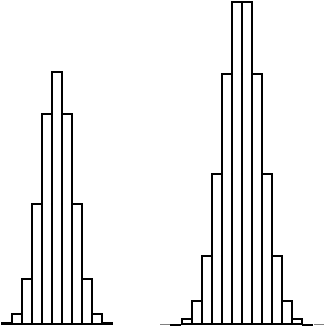
\includegraphics[scale=0.45]{FiguresMaths/ProbaGaussianDistribution}
        \caption{Histograms of the binomial coefficients in the $10$th row (left) and the $15$th row (right) of Pascal's triangle.  The righthand histogram has been scaled---in the proportion 1:20---in order to fit on the page.}
        \label{fig:gaussiandistribution}
\end{center}
\end{figure}

It is worth noting in Fig.~\ref{fig:gaussiandistribution} that the set of binomial coefficients
\[ \left\{ {n \choose k} \ | \ k = 0, 1, \ldots, n \right\} \]
hence, also the set of probabilities within a binomial distribution, has a single maximum when $n$ is even but {\em two} maxima when $n$ is odd.  This is important to keep in mind during analyses, so that one does not inadvertently miscount cases.


\subsubsection{Normal distributions; the {\em Central Limit Theorem}} 
\label{sec:normal-distr}

\index{normal distribution} \index{normal distribution!mean} \index{Gaussian distribution}
\index{normal distribution!variance} \index{normal distribution!standard deviation}

Although our focus is squarely on {\em discrete} mathematical phenomena, it is important to point out concepts and insights that emerge from related {\em continuous} phenomena.  This subsection and the next focus on two of the most important continuous probability distributions.

\medskip

The most familiar Bell curve probability distributions is the continuous {\em normal}, or, {\it Gaussian} distribution.  The term ``normal" here does not refer to a specific probability distribution but rather to a large family of distributions all of whose ``higher moments"---meaning all moments other than the mean and variance (or, equivalently, the standard deviation) are identically $0$.  Despite this rigorous specification, most non-statisticians identify a normal probability distribution as any one whose probability frequency function has the form
\[ f(x) \ = \ \frac{1}{\sqrt{2 \pi} \sigma} \ e^{\frac{(x - \mu)^2}{2 \sigma^2} } \]
In this formula: $\mu$ is the {\it mean} of the distribution, and
$\sigma^2$ (resp., $\sigma$) is its {\it variance} (resp., its {\it
  standard deviation}).  In this setting, the parameters $\mu$ and
$\sigma$ {\em specify} each individual normal distribution, which one
can unambiguously denote $ND(\mu, \sigma)$.  Many people focus on a
{\em standardized} normal distribution as the default, namely,
$ND(0,1)$; this distribution has the simpler form
\[ f(x) \ = \ \frac{1}{\sqrt{2 \pi}} \ e^{x^2/2} \]
To those who focus on the standardized normal distribution, $ND(0,1)$, as the
default, the more general familiy of distributions $ND(\mu, \sigma)$,
in the values of $\mu$ and $\sigma^2$ can be specified, is called a {\em generalized normal distribution}.  Of course, the values $\mu$ and $\sigma^2$ shift the specified Bell curve and change the slope of its ascent and descent.

\bigskip

\noindent \fbox{
\begin{minipage}{0.96\textwidth}
{\bf Cultural aside}.

\smallskip

Note that the normal probability frequency function involves two of the fundamental constants of mathematics: $e$ and $\pi$.  The ubiquity of these constants throughout disparate areas in mathematics testifies eloquently to how fully they deserve to be labeled {\em fundamental}.
\end{minipage}
}

\bigskip

\index{Central Limit Theorem} \index{de Moivre, Abraham}

The normal distribution is of immense importance in empirical studies of phenomena whose true distribution is unknown.  For such studies, the {\em Central Limit Theorem} of probability theory and statistics guarantees the following (stated informally).  Say that we design an experiment whose outcomes comprise the sample space of interest.  Say further that the trials from the experiment are mutually independent---so that their outcomes can be viewed as independently drawings of random variables from the sample space.  Then: {\em No matter how the original random variables are distributed---in particular, {\em they need not be distributed normally!}---the averages of the outcomes become normally distributed when the number of outcomes is sufficiently large. }

\bigskip

\noindent \fbox{
\begin{minipage}{0.96\textwidth}
$\oplus$ {\bf Enrichment note}.

\smallskip

For those readers who would like to see how one can formally state a sweeping result such as the Central Limit Theorem, we provide the following annotated semi-formal statement, of course without proof.

\begin{description}
\item[{\bf The Central Limit Theorem}]

\item{}

\item[{\sf Premise:}]
{\em Let $X_1$, $X_2$, \ldots, $X_n$ be random variables (over $\R$) which are all drawn from a distribution that has mean $\mu$ and finite variance $\sigma^2$.}

\smallskip

\medskip\item[{\sf Commentary:}]
Note that we do not demand any uniformity among the $X_i$ other than that they all come from {\em the same} distribution.  When these variables represent outcomes of distinct trials from the same experiment, this demand will be satisfied automatically.

\smallskip

\medskip\item[{\sf Conclusion:}]
{\em As the number of $X_i$, call it $n$, grows without bound---i.e., for sufficiently large values of $n$---the random variable}
\[ S_n \ = \ \frac{X_1 + X_2 + \cdots + X_n}{n} \]
{\em (which is the sample mean) converges to the actual mean $\mu$ of $ND(\mu, \sigma^2)$.}
\end{description}
\end{minipage}
}

\bigskip

\index{de Moivre, Abraham}

There are many versions of the Central Limit Theorem, which instantiate certain details of its premise in various ways.  The earliest version seems to date to a 1738 edition of {\it The Doctrine of Chances} \cite{DeMoivre}, the first text on probability theory.  In this major work, the French mathematician Abraham de Moivre conceived a brilliant idea while observing the pattern of the various summands in Newton's binomial formula (Theorem~\ref{thm:Binomial-theorem}).  He observed that as the Theorem expands the polynomial $(x+y)^n$, one can view what is happening as an analogue of quite a different manner of ``expansion".  (Recall our call in Chapter~\ref{ch:doingmath} to look for nonobvious, sophisticated patterns throughout the world.)  De Moivre noted that one can think of the polynomial being expanded as a $2$-event system that one is observing.  Viewed this way, the variables $x$ and $y$ become disjunctive sub-events of the compound event $x+y$; and the power $n$ becomes a measure of the number of observations that one has made.  This bold intuition suggests that {\em maybe}, over sufficiently many observations, one might observe the regularity in the $2$-event system that the Binomial Theorem guarantees in the bivariate polynomial.

\smallskip

\noindent
This intuition turns out to be correct---as verified by the Central Limit Theorem.

\bigskip

\noindent Back to the world of probability distributions \ldots

\medskip

\index{probability!distribution function} \index{probability!cumulative distribution function}

\noindent {\it  Cumulative distribution functions.}
In addition to the point-wise information that a probability frequency function yields, we are
often interested in the {\em cumulative} information yielded by the {\it (cumulative) distribution function}\footnote{Mathematicians usually refer to function $F$ simply as a distribution function; statisticians usually add the qualifier ``cumulative".}~$F$ on $S$, which is defined in one of the following dual forms for $x \in S$:
\[ F^{(\leq)}(x) \ = \ Pr[X \leq x] \ \ \ \ \mbox{ or} \ \ \ \  F^{(\geq)}(x) \ = \ Pr[X \geq x]\]

\smallskip

In {\em discrete} settings, cumulative distributions are usually defined via summation:
\[ F^{(\leq)}(x) \ = \ \sum_{y \leq x} \ f(y)  \ \ \ \ \mbox{ or} \ \ \ \ F^{(\geq)}(x) \ = \ \sum_{y \geq x} \ f(y) \]

\bigskip

The computational relation of a probability frequency function $f$ to its associated cumulative distribution functions can be quite complicated.  For one probability distribution that is very important in empirical studies of manifold phenomena, this relation is very simple.  We refer here to the so-called {\em exponential distributions.}


\index{exponential distribution}

\subsubsection{Exponential distributions} 
\label{sec:exponential-distr}

Distributions whose probabilities of success fall off at an exponential rate are roughly as familiar to experimenters as are normal distributions, because---as we shall discuss momentarily---such distributions are {\em memoryless}.

\medskip

\index{exponential distribution!decay rate}
\index{exponential distribution!probability frequency function}
\index{exponential distribution!cumulative frequency function}
A probability frequency function describes an exponential probability distribution just when there exists a {\em rate parameter}---traditionally denoted by $\lambda$---for which
\[ f(x) \ \eqdef \ Pr[X=x] \ = \ \lambda \cdot e^{-\lambda x} \]
The parameter $\lambda$ is often termed the {\em decay rate} of the distribution because of the behavior of the distribution's {\em cumulative frequency function} $F$---specifically its exponential drop-off, or, decay, with increasing $\lambda$.
\[ F(x) \ \eqdef \ Pr[X \leq x] \ = \ 1 - e^{-\lambda x} \]

\index{exponential distribution!mean}
\index{exponential distribution!variance} \index{exponential distribution!standard deviation}
\index{memoryless probability distributions} \index{conditional probabilty}

\medskip

The detailed derivations of the properties of the exponential distribution employ continuous mathematical concepts that are outside the scope of this discrete text.  But the properties themselves are worth mentioning, both for their (scientific and mathematical) cultural value and as an enticement to acquire the mathematical tools that will give access to this material, which is indispensable to empirical studies in computational domains.

\begin{prop}
\label{thm:exponential-moments}
For any exponentially distributed random variable $X$ with rate parameter $\lambda$:
\begin{enumerate}
\item
$\displaystyle \mbox{\sc mean}(X) \ = \ 1 / \lambda$.

\medskip\item
$\displaystyle \mbox{\sc variance}(X) \ = \ 1 / \lambda^2$.

\medskip\item
$\displaystyle  \mbox{\sc standard-deviation}(X) \ = \  \mbox{\sc mean}(X)$.

\medskip\item
The memoryless property:  For all $x, y \geq 0$,
\[ Pr[X > x+y \ \ | \ \ X > y] \ = \ Pr[X > x] \]
\end{enumerate}
\end{prop}

Note our invocation in Part 4 of {\em conditional} probabilities; cf., Section~\ref{sec:monty-hall}: We are concerned with the probability that the random variable $X$ exceeds the quantity $x+y$ {\em given that} $X$ exceeds the quantity $y$.


\subsection{A Historically Important Observational Experiment}
\label{sec:Arbuthnot}

An observational experiment that dates to the early 18th century played a historically significant role in the development of the operational methodology of the field of statistics.  The experiment arose from the curiosity of the 18th-century British polymath John Arbuthnot.
\index{Arbuthnot, John}

\smallskip

Arbuthnot's curiosity, so the story goes, was piqued by a popular belief of the period that more boys are born than girls.  In an effort to gauge the veracity of this belief, Arbuthnot studied an archive that he had access to, which reported on births in London in the $82$-year period 1629--1710.  As reported in his 1710 paper \cite{Arbuthnot}, Arbuthnot observed results such as the following (citing figures just from the first and last years that he reported on):\footnote{London's population was growing during this period, which accounts for the roughly $50\%$ growth in the total number of births.}
\begin{itemize}
\item
In 1629, male births were $52.7\%$ of the total: 5218 males versus 4683 females;
\medskip\item
in 1710, male births were $51.8\%$ of the total: 7640 males versus 7288 females.
\end{itemize}
In fact, to Arbuthnot's surprise, the archives exposed that male births consistently outnumbered female births throughout the $82$ years covered by the archives!

\smallskip

Roughly a century after Arbuthnot, the French mathematician Pierre Simon Laplace---who invented much of the mathematics underlying probability and statistics---reported in \cite{Laplace} that the total number of male births outnumbered the total number of female births in the proportion of roughly $22$ ($51.2\%$) to $21$ ($48.8\%$).
 \index{Laplace, Pierre Simon}

\medskip

\noindent
So \ldots \ \ Are male births actually more common than female births?

\medskip

\noindent
Arbuthnot would have responded YES to this query, based on the following reasoning, which is inspired by how one would analyze a coin-tossing experiment.  If the ``coin" is unbiased---so that the genders-of-newborns observations are reporting on a random process with two equiprobable outcomes---then we would expect to see each new birth be a male or a female with probability $1/2$.  Over the course of $82$ years, with (very roughly) $10,000$ births per year, then, the probability of seeing more boys than girls should equal $p=(1/2)^{820,000}$, which should be {\em very} close to $0$.  The fact that he observed more male births than female births over the entire period of his observations therefore convinced Arbuthnot that he was observing a true deviation from randomness---i.e., there {\em is} an actual bias toward male births!

\medskip

Would we draw the same conclusion today as Arbuthnot did roughly three centuries ago?  Is the probability $22/43 \approx 0.512$ of male births that Laplace observed sufficiently larger than the random expectation $1/2 = 0.5$ for us to reject the hypothesis that this deviation could be pure chance?

\medskip

{\em This is precisely the kind of question that the field of statistics specializes in!}

\subsection{The Law of Large Numbers}
\label{sec:Large-Numbers}

\index{Law of Large Numbers} \index{{\it Loi des grands nombres}}

An operationally sound answer to the Arbuthnot-Laplace question can be derived from a second major probability-related theorem.  This result, which is known as the {\it Law of Large Numbers}, or, {\it la Loi des grands nombres}, focuses on the sequence of random variables $\langle S_1, S_2, \ldots \rangle$, where each $S_n$ is the average of the first $n$ observed outcomes from an experiment of interest.  The Law asserts that the variables $S_n$ tend progressively closer to (i.e., {\em converge to}) the actual idealized mean of all possible outcomes of the experiment---no matter how the outcomes are distributed probabilistically.  Said differently: {\em The more times one repeats a random experiment, the more closely the observed outcomes trend toward the actual mean outcome:  Repetition improves accuracy!}

\medskip

The {\it Law} and the {\it Central Limit Theorem} are really kindred results.  Both yield information about the sums of random variables, which is as significant in practice as it is interesting mathematically, and both yield to essentially the same formal reasoning.  Of course, the Law is really the weaker of the two results, in that it yields guarantees only about the {\em means} of sums of random variables, whereas the Theorem yields guarantees about the sums' {\em variances} also.

\bigskip

\noindent \fbox{
\begin{minipage}{0.96\textwidth}
$\oplus$ {\bf Enrichment note}.

\smallskip

As we did with the Theorem, we provide the following annotated semi-formal statement of the sweeping Law of Large Numbers.

\begin{description}
\item[{\bf The Law of Large Numbers}]

\item{}

\item[{\sf Premise:}]
{\em Let $X_1$, $X_2$, \ldots, $X_n$ be random variables which are all drawn from a distribution that has mean $\mu$.}

\medskip\item[{\sf Commentary:}]
The Law and the Central Limit Theorem make similar demands on their inputs.

\medskip\item[{\sf Conclusion:}]
{\em As the number $n$ of $X_i$ grows without bound---i.e., for sufficiently large values of $n$---the random variable}
\[ S_n \ = \ \frac{X_1 + X_2 + \cdots + X_n}{n} \]
{\em (which is the sample mean) converges to the actual mean $\mu$.}
\end{description}
\end{minipage}
}

\bigskip

\index{von Bielfield, Jakob} \index{Bernoulli, Jacques (Latin: Jacobi)} \index{Bernoulli, Nicholas}

Much of our knowledge about the early history of the Law is due to the 1767 book on statistics by the prolific German writer Jakob von Bielfeld.  The Law first appears as a theorem in the 1713 book \cite{Bernoulli} by the Swiss mathematician Jacques (Latin: Jacobi) Bernoulli.  Because of Bernoulli's death, this work was completed by his nephew Nicholas, and the book was published posthumously (the notation {\it ``opus posthumum"} in the citation). 

\medskip

We illustrate the Law via simple examples before returning to the Arbuthnot-Laplace question.

\begin{enumerate}
\item
We know the probabilistic behavior of experiments involving rolls of two $6$-sided dice.  Since each of the six outcomes is equiprobable for each die, we can argue that as we roll the pair many times, we expect to see the {\em average} outcome
\[ \frac{1+2+3+4+5+6}{6} \ = \ 3.5 \]
Of course, we cannot expect to see this average roll by roll---that is why we need higher moments to truly understand the behavior of experiments!  But the Law guarantees that as we roll the dice over and over, we should observe the sequence of average roll-values tending to $3.5$.

\medskip\item
Let play an illustrative (but uninteresting) ``game" using a barrel that contains both white and black balls.  We will repeatedly draw a ball from the barrel, record its color, and replace the ball.  What will our records show about the relative numbers of black and white balls we shall observe.

\smallskip

Say for illustration that the barrel contains 300 white balls and 200 black balls, for a $60\%$--$40\%$ split.

\smallskip

Clearly, there is always a greater chance of pulling a white ball from the barrel than a black ball.  But, the Law of Large Numbers tells us quite a bit more:  It tells us that as we play the ``game" for longer and longer, the probability of drawing a white ball will get closer and closer to $60\%$.

\medskip

Let us put this result in perspective.

\smallskip

Of course, if we draw only a single ball---a single trial in the ``game"---then the result is simply either $1$ white ball and $0$ black balls or vice versa.  It is only after many trials that we will encounter interesting tallies. How many trials do we have to do before we begin to see the probability of a white ball edge up toward $60\%$?  Will we observe close to $60\%$ white balls after $10$ trials? $100$ trials? $1000$ trials?  In fact the proof of the Law will answer this question, to within whatever {\it level of confidence} we want!  If, for instance, we want to be sure to draw white balls with a probability between $59.9\%$ and $60.1\%$, i.e., with a confidence level of $1\%$, then the analysis underlying the Law will tell us how many trials we have to do to achieve this.

\smallskip

As an aside, in commercial applications, a $5\%$ confidence level is often considered an acceptable compromise between the (probabilistic) guarantee of the Law and the work required to achieve that guarantee.
\end{enumerate}

\ignore{******************
{\Arny I have changed my mind about the {\sc select-and-replace} game.  I now propose that we use it as an exercise.  The following writeup also contains the solution, so it should be easy to port to the EXERCISE section, if you agree with my assessment.}

{An Illustrative Game}

The following simple game illustrates probability frequency functions and
gives us access to other important probability-related functions.

The {\sc select-and-replace} game is played by a single-player $P$, using a
set $\Sigma$ of $n$ tokens, labeled $1$, $2$, \ldots, $n$; set $\Sigma$
also serves as our sample space. (The important thing in this setting is that 
the token labels are distinct, not that they comprise the first $n$ integers.)
Each move of the game has $3$ stages.  In each move, player $P$:

(1) {\em removes a token from set $\Sigma$};

(2) {\em records the label of the removed token};

(3) {\em replaces the token into set $\Sigma$}.

\noindent
At the end of the $n$ moves, we assign player $P$ a score that is the number of 
{\em distinctly labeled} tokens that $P$ had removed (and replaced) over the
course of this $n$-move play of the game.  (Even if $P$ removes and replaces
a given token $\tau \in \Sigma$ multiple times, token $\tau$ counts only once toward $P$'s score.)

Let us denote by $X$ the random variable which assumes the value 
$k \in \{1, 2, \ldots, n\}$ on a particular play of the {\sc select-and-replace} game 
just when player $P$ achieves score $k$ during that play.  We can calculate the
probability $Pr(k)$ of achieving score $k$ by directly invoking the
definitional ratio (\ref{eq:prob-def-ratio}).  We argue using basic facts involving 
binomial coefficients.
\begin{itemize}
\item
For each integer $k$, $\displaystyle {n \choose k}$ is the number of ways to 
select $k$ items from a set of $n$ items.
Hence, it is also the number of $k$-elements subsets of the $n$-element 
set $\Sigma$.
\medskip\item
The binomial coefficients with upper argument $n$ sum to $2^n$:
\[ \sum_{k=0}^n \ {n \choose k} \ = \ 2^n \]
Hence, $2^n$ is the total number of subsets of the $n$-element set $\Sigma$,
and $2^n -1$ is the number of {\em nonempty} such sets.
(We already knew this, of course.)
\end{itemize}
Thus, $P$'s score can result from selecting any of $\Sigma$'s $(k > 0)$-element 
subsets---which are $\displaystyle {n \choose k}$ in number---from among 
$\Sigma$'s $2^n -1$ nonempty subsets.  It follows, therefore, that
\[ Pr(k) \ \eqdef \ Pr[X = k] \ = \ {n \choose k} \div (2^n -1)  \]

By definition, $Pr(x)$ is a probability frequency function for random variable $X$.
*****************}

\medskip

We return briefly to the Arbuthnot--Laplace question in the light of the Law of Large Numbers.  Laplace's calculation of $22/43$ as the ratio of male births to total births was based on literally hundreds of thousands of births.  It is {\em highly unlikely}, therefore, that male births did not exceed female births, at least in the London of the period 1629--1710 ,by the ratio $22$ to $21$.

\medskip

\noindent
Interestingly the gender imbalance in births exposed by Arbuthnot can still be observed today---we are not sure what the current ratio is---and the reason for the imbalance has not yet been clearly identified.

\subsection{Statistical Tests}
\label{sec:stat-tests}

\index{statistical tests}

We close our introductory survey of mathematical statistics by informally introducing the important topic of {\em statistical tests}.  Such tests are most laypersons' most intimate connection with the field of statistics.  The tests enable us to determine whether distinct streams of observed experimental outcomes are positively correlated.  As but two illustrations, tests enable us to recognize:
\begin{itemize}
\item
a positive correlation between negative reactions to a pharmaceutical and the strength of prescribed doses.  
\medskip\item
the fact that the observed diameters of roller bearings in a manufacturing run do not belong to the planned statistical distribution.
\end{itemize}
In its simplest form, such a test often just asks whether observed values come from similarly distributed random variables.

\medskip

The topic of statistical testing is enormous and mostly beyond the scope of any introductory text (certainly an introductory mathematics text).  The reader who wants a comprehensive introduction to statistical testing, especially from a mathematical perspective, is referred to a text such as \cite{Hoel58}.   We introduce here just a single approach to testing---via {\em distance metrics}.  This approach employs three intertwined conceptual steps.
\begin{enumerate}
\item
One computes an appropriate measure of {\em distance} between the two target sequences of observations.
\medskip\item
The ``appropriateness" of a particular distance metric presupposes our ability to associate probabilities with specific observed distances.

\smallskip

Therefore, one must analyze the distribution(s) that the sequences come from, to determine the probability that two targeted sequences will achieve a particular observed inter-sequence distance.
\medskip\item
One selects a {\em confidence level} to determine whether the observed probability that the targeted sequences are related is large enough for us to accept them as related in the sense of interest.

\medskip

Confidence levels are another way to look at probabilities.  To wit, the statement

\hspace*{.2in}{\em the probability that the assertion $A$ is true is $p\%$}

is equivalent to the statement

\hspace*{.2in}{\em assertion $A$ is true with a confidence level of $(100-p)\%$}.
\end{enumerate}

\bigskip

\noindent \fbox{
\begin{minipage}{0.96\textwidth}
{\bf Explanatory note}.

\smallskip

Traditionally:
\begin{itemize}
\item
The statement which asserts that the observed sequence and the expected sequence come from the same distribution is called the ``{\em null hypothesis}".

\medskip\item
Accepting the proposition that the targeted sequences are related is termed ``{\em accepting the null hypothesis}".
\end{itemize}
\end{minipage}
}

\subsubsection{Testing means in binomial distributions}

We can illustrate the described test-implementation steps by returning briefly to the Arbuthnot-Laplace question of Section~\ref{sec:Arbuthnot}.   In that section, we dealt with this question in a rather informal manner.  With a more formal testing regimen, we could end up with a statement such as the following.

\smallskip

\begin{tabular}{l}
{\em To within the confidence level $c$} (choose a number here) {\em the London records} \\
{\em demonstrate that there were more male births than female births in the} \\
{\em $82$-year period period 1629--1710.}
\end{tabular}

\smallskip

\noindent
We would develop this more formal statement by studying the Arbuthnot-Laplace question within the framework of statistical testing, in the following manner.
\begin{itemize}
\item
The target sequences of interest have length $82$, corresponding to the $82$ years of births that the London records report on. 
\medskip\item
For each $i \in \{1,2, \ldots, 82\}$:

\smallskip

The $i$th entry in the {\em observed} sequence $\langle o_1, o_2, \ldots, o_{82} \rangle$ reports on the {\em observed} fraction of male births for year $i$ of the $82$-year stretch.

\smallskip

Every entry in the {\em expected} sequence $\langle e_1, e_2, \ldots, e_{82} \rangle$ is ``$e_i \equiv 1/2$", for this is what the observed fraction {\em would be} if there were no disparity in the relative numbers of male and female births.

\medskip\item
If we assume---as Arbuthnot did---that the birth patterns of males and females obeys a binomial distribution, then our analysis in Section~\ref{sec:binomial-distribution} would provide the probabilities of the various possible ratios of male and female births.  Table~\ref{tab:select-replace} provides concrete values for these probabilities for the cases $n=10$ and $n=15$.

\medskip\item
Since we are interested only in means rather than more highly structured distributions, we can choose a simple metric to measure the distance between the observed and expected sequences.  We choose the metric adapted from the $L^2$-norm of Section~\ref{sec:Ln-norms}, i.e., the distance
\[ {1 \over 82} \sum_{i=1}^{82} \ (o_i -e_i)^2 \ = \ {1 \over 82} \sum_{i=1}^{82} \ (o_i - 1/2)^2 \]

\medskip\item
We can now choose a confidence level $c$, which would give one access to the desired formal statement.
\end{itemize}

\subsubsection{The $\chi^2$ test for multinomial distributions}
\index{multinomial distributions}

Probability theory and statistics do not restrict themselves to simple metrics or simple distributions.  Once one allows even moderately more sophisticated distributions, a whole range of important practical situations can be discussed and analyzed.
 \index{statistical tests!the $\chi^2$ test} 

\medskip

The {\it $\chi^2$ test} is a statistical test which allows one to test whether two sequences of values come from the same {\em multinomial distribution}---a generalization to many variables of the binomial distribution that we studied in Section~\ref{sec:binomial-distribution}.  In contrast to the $L^2$-distance measure that we used to analyze the Arbuthnot-Laplace question, we now discuss a more ambitious question, and, accordingly, invoke a stronger statistical test.

\smallskip

As before, we begin with two sequences that can be viewed as representing either $m$ trials of an experiment or $m$ sample values drawn from a given sample space:  There is the sequence 
\[ \langle e_i \rangle_{i=1}^m \ \ \eqdef \ \ \langle e_1, e_2, \ldots, e_m \rangle \]
of {\em expected} values and the  sequence
\[ \langle o_i \rangle_{i=1}^m \ \ \eqdef \ \ \langle o_1, o_2, \ldots, o_m \rangle \]
of {\em observed} values.  We seek to determine the probability that both sequences arise from sampled values from the same random variable.

\smallskip

The $\chi^2$ test measures the distance between sequences $\langle e_i \rangle_{i=1}^m$ and $\langle o_i \rangle_{i=1}^m$ via a calculation that can be viewed as the {\em relative error} incurred by trying to pass either of these sequences off as the other.  Specifically, the $\chi^2$ distance/error corresponding to these sequences is
\[ \chi^2 \ = \ \sum_{i=1}^m \ \frac{(o_i- e_i)^2}{e_i} \]
The $\chi^2$ test invokes an analysis of the relevant {\em multi}nomial distribution---analogous to our analysis of the {\em bi}nomial distribution---to calculate the probability that the observed and expected sequences come from the same multinomial distribution.

\medskip

We illustrate the domain of the test via a simple illustrative example that we excerpt from \cite{Hoel58}.

\bigskip

We roll a ($6$-sided, allegedly fair) die $60$ times.  We expect to
see $10$ occurrences each of the $6$ possible outcomes.  The $\chi^2$ test computes the distance between the following sequences:
\[ \begin{array}{|l||c|c|c|c|c|c|}
\hline
\mbox{60 Rolls of a die}  &
\mbox{Face } \#1 &
\mbox{Face } \#2 &
\mbox{Face } \#3 &
\mbox{Face } \#4 &
\mbox{Face } \#5 &
\mbox{Face } \#6 \\
\hline \hline 
\mbox{Observed frequencies:}
  & f_1 & f_2 & f_3 & f_4 & f_5 & f_6 \\
\hline
\mbox{Expected frequencies:}
  & 10 & 10 & 10 & 10 & 10 & 10 \\
\hline
\end{array}
\]
The test then calculates the probability $p$ that the observed sequence, $\langle f_1$, $f_2$, $f_3$, $f_4$, $f_5$, $f_6 \rangle$ comes from the same multinomial distribution as does the expected sequence $\langle 10, 10, 10, 10, 10, 10 \rangle$. 

\smallskip

As usual, one selects a confidence level $c$, which is equal to $1-p$, and one announces that, to within the confidence level $c$, the observed sequence $\langle o_i \rangle_{i=1}^{60}$ does come from the same distribution as the expected sequence $\langle e_i \rangle_{i=1}^{60}$.

\smallskip

If the confidence level $c$ must be chosen too high before it mandates accepting the null hypothesis, then one could decide that the rolled die is not fair!  This is the way that our setting can be used in applications such as fault analysis and quality analysis.


\ignore{**************
\subsection{Pointers to Advanced Topics}
\label{sec:advanced-stat}

This chapter has presented the tools needed to understand the ethos of the field of statistics and to plant the seeds for an operational understanding of the field.  The two probabilistic-statistical ``blockbusters" that we have discussed, the Central Limit Theorem and the Law of Large Numbers, point the way to further topics in the field of mathematical statistics, that are more specialized and/or more advanced.  We close the section with two subsections that introduce some of this material that is beyond the scope of this text.


In Section~\ref{sec:advanced-stat}, we provide thumbnail sketches of advanced topics in statistics which are essential for the mastery of computational applications whose relevance to daily life increases almost day to day.  


OTHER topics that relate to this chapter but are too advanced and/or specialized for inclusion in this text.

As students are introduced to modern topics within computing, whether at the level of a Computing Literacy course or a post-core technical course, they will have to master a variety of more specialized topics that combine pieces of the elements we have discussed in this essay.
While these topics are beyond the level of generality aimed at in this essay, some may be appropriate prerequisites to programs that have some specialized foci.
\begin{itemize}
\item
Issues relating to {\em clustering} according to various affinity measures find application in applications as diverse as: {\em linear-algebraic computations}, {\em data mining}, {\em design and layout of digital circuitry}.


\medskip\item
Many issues relating to {\em fault/failure tolerance} and {\em data analytics} benefit from study using {\em random walks} (at least in one dimension).
\end{itemize}

The preceding list is really endless.  Hopefully readers will be inspired by our few examples to compile a longer version that is appropriate for their particular environments.
*************}

%%%%%%%%%%%%%%%%%%
\section{Exercises: Chapter 11}

Throughout the text, we mark each exercise with 0 or 1 or 2 occurrences of the symbol $\oplus$, as a rough gauge of its level of challenge.  The 0-$\oplus$ exercises should be accessible by just reviewing the text.  We provide {\em hints} for the 1-$\oplus$ exercises; Chapter~\ref{ch:Exercises} provides {\em solutions} for the 2-$\oplus$ exercises.  Additionally, we begin each exercise with a brief explanation of its anticipated value to the reader.

\begin{enumerate}
\item
{\bf Counting arrangements}

{\sc Lesson:} Experience with combinatorial calculations

  \begin{enumerate}
  \item
{\bf Counting repetitions}

\smallskip

{\em Prove Proposition~\ref{thm:identical-events}:

The number of possible outcomes when a fair $6$-sided die is rolled $n$ times is $6^n$.}

  \medskip\item
{\bf Counting permutations}

\smallskip

{\em Prove Proposition~\ref{thm:no-permutation}:
The number of permutations, $P(n)$, of a $n$-element set equals $n!$}

  \medskip\item
{\bf Counting arrangements}

\smallskip

{\em Prove that the number of ways of selecting $k$ unordered items out of a set of $n$ items is $\displaystyle {n \choose k}$.  Your proof must be based on Proposition~\ref{thm:no-permutation}.}
  \end{enumerate}

\medskip\item
$\oplus$
{\bf Counting replicated triangles}

{\sc Lessons:} Experience with detecting sophisticated patterns and using recurrences.

\smallskip

Let us begin with a single isosceles triangle, call it $T_1$, as in Fig.~\ref{fig:countingTriangles}(left).
\begin{figure}[h]
\begin{center}
        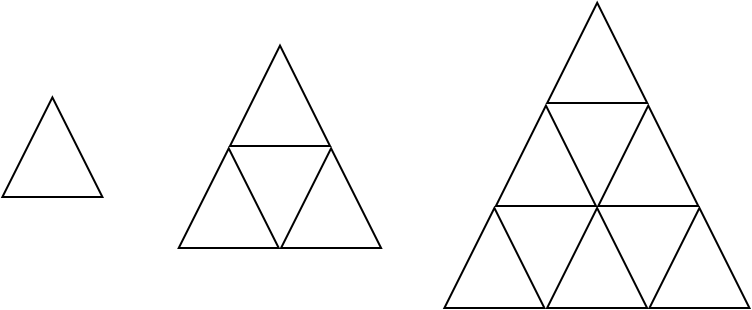
\includegraphics[scale=0.35]{FiguresArithmetic/CountingTriangles}
        \caption{The first three stages of triangle-replication.}
        \label{fig:countingTriangles}
\end{center}
\end{figure}

Next, let us create the isosceles triangle $T_2$ of Fig.~\ref{fig:countingTriangles}(center) by taking four copies of $T_1$ and placing them together in the manner depicted in the figure. 
Now, $T_2$ is similar to $T_1$, in the geometric sense of the word, and its height and base are twice those of $T_1$.  
What really interests us, though, is that the {\em drawing} of $T_2$ in the figure contains {\em five} triangles---namely, the four copies of $T_1$ {\em plus} the isosceles triangle that contains these four copies.

As our next step, we iterate the replication process by append to $T_2$ an additional layer consisting of five copies of $T_1$ arranged as indicated in Fig.~\ref{fig:countingTriangles}(right).  
The resulting isosceles triangle, $T_3$, has a base and a height that are three times those of $T_1$.  
Once again, what really interests us is that the {\em drawing} of $T_3$ in the figure contains {\em thirteen} triangles---namely, the four copies of $T_1$ {\em plus} the isosceles triangle that contains these four copies.  
Specifically, we can discern {\em nine} copies of $T_1$, 
{\em three} copies of $T_2$, {\em plus} the all-encompassing big isosceles triangle.

Of course, we can now append to $T_3$ an additional layer consisting of seven copies of $T_1$, and we can then append an additional layer consisting of nine copies of $T_1$, and on and on.
\smallskip

As we make these successive augmentations, how does the progression of numbers of triangles grow?
It is clear that there is a recurrence lurking here.  
Your challenge is to discover it.  
To this end, let $N_k$ denote the number of triangles within triangle $T_k$.  
We have just seen that $N_1 =1$, $N_2 = 5$, and $N_3 = 13$.
  \begin{enumerate}
  \item
$\oplus$
{\em Compute} $N_4$.
  \medskip\item
$\oplus \oplus$
{\em Develop a recurrence for} $N_k$ (i.e., the general case).
  \end{enumerate}

%%%

\medskip\item
{\bf More about birthdays}

{\sc Lesson:} Experience with combinatorial probability

\smallskip

  \begin{enumerate}
  \item
{\em Determine the probability that a person you meet on the street was born on February 28.}
  \medskip\item
{\em Determine the probability that a person you meet on the street was born on February 29.} 
  \medskip\item
{\em Find a number $n$ that satisfies the following.  With probability at least $1/2$, any collection of $n$ people contains $\geq 3$ people who share the same birthday}.
  \end{enumerate}  
  
%%%

\medskip\item
$\oplus$
{\bf Further analysis of poker hands}

{\sc Lessons:} Experience analyzing simple combinatorial situations

\smallskip

{\em Determine the probability of being dealt a two-pair hand in a fair game of poker.}

\smallskip

{\em Hint}.  As noted in the text, a two-pair hand is any permutation of
\[ X, \ X, \ Y, \ Y, \ Z \]
where $X$, $Y$, and $Z$ are distinct face-values.  If you try to pick these three values separately, you will be subjecting yourself to a complex case analysis.  You are much better off to select the three distinct values from the $13$ possible face-values in a single conceptual step.  Then you must select which of the three face-values will play the role of $Z$ (the unpaired card). 
At that point, you should be well on your way to the answer!

%%%

\medskip\item
{\bf Further analysis of simple dice-rolling games}

{\sc Lessons:} Experience analyzing simple combinatorial situations

\smallskip

  \begin{enumerate}
  \item
{\em Analyze the game of craps in the same way as we did for the (unordered) sum-of-three game.}

  \medskip\item
One notes in Fig.~\ref{fig:dice-ordered-configs} that In the ordered version of the sum-of-three game, the sum $k$ is engendered by the same number of configurations as is the sum $21 - k$.  
{\em Explain why this is true.}
  \end{enumerate}
  
%%%

\smallskip
\medskip\item
{\bf Some statistical calculations}

{\sc Lesson:} Experience with combinatorial calculations

\smallskip
  
{\em Prove Proposition~\ref{thm:mean-linear}, which asserts the linearity of the mean.}

%%%

\medskip\item
{\bf Monge shuffles: mathematical party tricks}

{\sc Lesson:} Experience with analyzing combinatorial patterns

\smallskip

\index{Monge, Gaspard} \index{Monge shuffle}

We consider two ways of shuffling cards which are associated with the 18-19th century French mathematician Gaspard Monge.  We employ the shuffle-techniques as vehicles for honing your skills in detecting combinatorial patterns.  Others have used them as party tricks.

\smallskip

For both shuffle-techniques. we begin with a deck of $2n$ distinct cards.  We employ the running example of the following small deck, where $n=4$:
\[ (1, \ 2, \ 3, \ 4, \ 5, \ 6, \ 7, \ 8) \]
For both {\it Monge shuffles} of the cards, we cut the deck in the middle, to create two $n$-card decks:
\[ (1, \ 2, \ 3, \ 4), \ (5, \ 6, \ 7, \ 8) \]
We then merge the two $n$-card decks to again obtain a single $2n$-card deck.  The two Monge shuffles differ in their merging techniques.

  \begin{enumerate}
  \item $\oplus$ {\bf The simple Monge shuffle}

\smallskip

The first, simple, Monge shuffle alternates the ``top" cards from the righthand and lefthand $n$-card decks; see Fig~\ref{fig:suffleMonge}.  The merged deck has the form
\[ (5, \ 1, \ 6, \ 2, \ 7, \ 3, \ 8, \ 4) \]
\begin{figure}[h]
\begin{center}
        \includegraphics[scale=0.4]{FiguresArithmetic/suffleMongeBasic}
        \caption{The Monge shuffle for $8$ cards ($n=4$).}
        \label{fig:suffleMonge}
\end{center}
\end{figure}

In the party-game incarnation of the Monge shuffle, you demonstrate the cut-then-merge process of Fig~\ref{fig:suffleMonge}, and you suggest to your audience that this process is a good first step in really mixing up the cards.  If this were so, then repeating the step several times should be a good way to obtain a ``random" mixture of the cards.

\smallskip

Let's see what happens after several steps of this cut-then-merge process:
\[ \begin{array}{ccccccccccccccccc}
(1 & 2 & 3 & 4 & 5 & 6 & 7 & 8) & \rightarrow & (1 & 2 & 3 & 4) & (5 & 6 & 7 & 8) \\
 & & & & & & & & \swarrow & & & & & & & & \\
(5 & 1 & 6 & 2 & 7 & 3 & 8 & 4) & \rightarrow & (5 & 1 & 6 & 2) & (7 & 3 & 8 & 4) \\
 & & & & & & & & \swarrow & & & & & & & & \\
(7 & 5 & 3 & 1 & 8 & 6 & 4 & 2) &  \rightarrow& (7 & 5 & 3 & 1) & (8 & 6 & 4 & 2) \\
 & & & & & & & & \swarrow & & & & & & & & \\
(8 & 7 & 6 & 5 & 4 & 3 & 2 & 1) &  \rightarrow& (8 & 7 & 6 & 5) & (4 & 3 & 2 & 1) \\
 & & & & & & & & \swarrow & & & & & & & & \\
(4 & 8 & 3 & 7 & 2 & 6 & 1 & 5) &  \rightarrow& (4 & 8 & 3 & 7) & (2 & 6 & 1 & 5) \\
 & & & & & & & & \swarrow & & & & & & & & \\
(2 & 4 & 6 & 8 & 1 & 3 & 5 & 7) &  \rightarrow& (2 & 4 & 6 & 8) & (1 & 3 & 5 & 7) \\
 & & & & & & & & \swarrow & & & & & & & & \\
(1 & 2 & 3 & 4 & 5 & 6 & 7 & 8)
\end{array}
\]
So, this does not look too random!  After {\em three} (which, ``coincidentally", equals $n-1$) cut-then-merge steps, the deck has been reversed, and after $2n-1$ cut-and-merge steps, it has been replicated in its original order!

\smallskip

As mathematicians, we do not like ``coincidences"!

\medskip

{\em Prove the following assertion.}

\begin{prop}
Let $p$ be a prime ($p>2$), and let $n = {1 \over 2} (p-1)$.  Let us begin with a deck of $2n$ distinct cards and perform the simple Monge shuffle on the deck.  After some number $m$ of cut-then-merge steps, where $m$ divides $p-1$, the simple Monge shuffle replicates the initial deck.
\end{prop}

Studying our sample sequence of cut-then-merge steps should provide a valuable hint.

\medskip

  \item $\oplus \oplus$ {\bf The sophisticated Monge shuffle}

\smallskip

We now provide a more sophisticated merge procedure, which yields a sophisticated variant of the Monge shuffle.  In each stage of this variant---each corresponding to a cut-then-merge step of the simple shuffle---we rearrange the $2n$-card deck directly, from the middle outward, via the following regimen:

\smallskip

\noindent
- Card \#1 of the original deck is placed in position $n+1$ of the shuffled deck \\
- Card \#2 of the original deck is placed in position $n$ of the shuffled deck \\
- Card \#3 of the original deck is placed in position $n+2$ of the shuffled deck \\
- Card \#4 of the original deck is placed in position $n-1$ of the shuffled deck \\
\hspace*{.1in} \ldots and so on, until the original deck is empty.

\smallskip

The first few steps of a stage of the sophisticated Monge shuffle are illustrated for the case $n=4$ in Fig.~\ref{fig:suffleMonge1};
\begin{figure}[h]
\begin{center}
        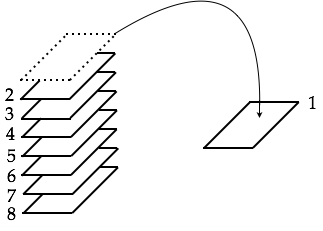
\includegraphics[scale=0.33]{FiguresArithmetic/suffleMongeStep1}
        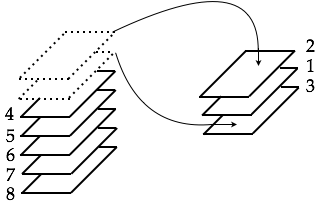
\includegraphics[scale=0.33]{FiguresArithmetic/suffleMongeStep2}
         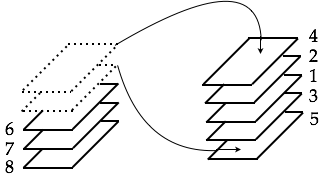
\includegraphics[scale=0.33]{FiguresArithmetic/suffleMongeStep3}
        \caption{The Monge shuffle for $8$ cards ($n=4$): Step 1 (left), Step 2 (center), Step 3 (right).}
        \label{fig:suffleMonge1}
\end{center}
\end{figure}
\ignore{**********
\begin{figure}[h]
\begin{center}
        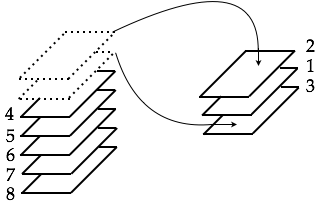
\includegraphics[scale=0.4]{FiguresArithmetic/suffleMongeStep2}
        \caption{Step 2. The Monge shuffle for $8$ cards ($n=4$).}
        \label{fig:suffleMonge2}
\end{center}
\end{figure}
\begin{figure}[h]
\begin{center}
        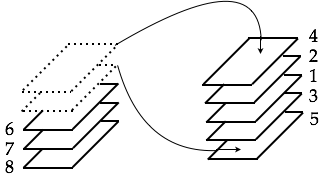
\includegraphics[scale=0.4]{FiguresArithmetic/suffleMongeStep3}
        \caption{Step 3. The Monge shuffle for $8$ cards ($n=4$).}
        \label{fig:suffleMonge3}
\end{center}
\end{figure}
***********}
One complete stage is illustrated in the table following the figure.
\[ \begin{array}{cccccccccccccccccc}
\mbox{Step } & \multicolumn{8}{c}{\mbox{Original deck}} & &
     \multicolumn{8}{c}{\mbox{Shuffled deck}} \\
\hline
1 & (1 & 2 & 3 & 4 & 5 & 6 & 7 & 8) & \rightarrow & ( - & - & - & - & 1 & - &  - & - ) \\
2 & ( - & 2 & 3 & 4 & 5 & 6 & 7 & 8) & \rightarrow & ( - & - & - & 2 & 1 & - & - & - ) \\
3 & ( - & - & 3 & 4 & 5 & 6 & 7 & 8) &  \rightarrow& ( - & - & - & 2 & 1 & 3 & - & - ) \\
4 & ( - & - & - & 4 & 5 & 6 & 7 & 8) &  \rightarrow& ( - & - & 4 & 2 & 1 & 3 & - & - ) \\
5 & ( - & - & - & - & 5 & 6 & 7 & 8) &  \rightarrow& ( - & - & 4 & 2 & 1 & 3 & 5 & - ) \\
6 & ( - & - & - & - & - & 6 & 7 & 8) &  \rightarrow& ( - & 6 & 4 & 2 & 1 & 3 & 5 & - ) \\
7 & ( - & - & - & - & - & - & 7 & 8) &  \rightarrow& ( - & 6 & 4 & 2 & 1 & 3 & 5 & 7 ) \\
8 & ( - & - & - & - & - & - & - & 8) &  \rightarrow& ( 8 & 6 & 4 & 2 & 1 & 3 & 5 & 7 ) \\
\end{array}
\]


\ignore{**********
Take the first card on top of the deck,
then, place the second one above, 
the third card below the two first ones, and so on alternatively
until the initial deck becomes empty.
Below is the decomposition of the first step:
Fig.~\ref{fig:suffleMonge1},~\ref{fig:suffleMonge2},~\ref{fig:suffleMonge3} show pictorially the three first steps of the process for $n=4$.


\medskip

{\em Prove the following properties of the sophisticated Monge shuffle.} 

\begin{enumerate}
\item Show that for $n=5$ the card at the fourth position remains fixed.
Is it still true for odd $n$?
\item Show that for any $n$ the initial order always appears once again.
In particular, how many steps are required for $n=12$?
\item Generalize the previous results:
for $n=3k+2$ prove that the card in position $k+1$ always remains unchanged.
\item For some values of $n$, show that there exist two cards that are always exchanged. Apply this to $n=11$.
\end{enumerate}
************}

\medskip

{\em Prove the following assertion.}

\begin{prop}
For any integer $n \in \N^+$: 
If $4n+1$ is prime, then performing $2n$ steps of the sophisticated Monge shuffle on a deck of $2n$ distinct cards restores the deck to its original order.
\end{prop}
  \end{enumerate}

\end{enumerate}

